\documentclass[12pt]{article}
\usepackage{pifont}
\usepackage{a4wide}
\usepackage[utf8x]{inputenc}
\usepackage{amsmath}
\usepackage{amsfonts}
\usepackage{mathrsfs}
%\usepackage{natbib}
\usepackage{graphicx} % figuras
%\usepackage[export]{adjustbox} % loads also graphicx
\usepackage{float}
\usepackage[font=footnotesize]{caption}
\usepackage{wrapfig}
\usepackage{authblk}
\usepackage{subfigure}
\usepackage{setspace}
\usepackage{amssymb}
\usepackage{latexsym}
\usepackage{footnote}
\usepackage[sort&compress]{natbib}



\topmargin=-2pt
\title{POD-based deflation techniques for the solution of two-phase flow problems in large and highly heterogeneous porous media.}

\author[1]{G. B. Diaz Cortes}  
\author[1]{C. Vuik} 
\author[2]{J. D. Jansen} 
\affil[1]{Department of Applied Mathematics, TU Delft}
\affil[2]{Department of Geoscience \& Engineering, TU Delft}
\renewcommand\Authands{ and }
\date{}


\begin{document}
\thispagestyle{empty}
\noindent
\begin{center}
{\Large \sc DELFT UNIVERSITY OF TECHNOLOGY}
\\
\vspace{3cm}
{\large \sc REPORT 18-01}\\[4ex]
{\large \sc POD-based deflation techniques for the solution of two-phase flow problems in large and highly heterogeneous porous media.}\\[4ex]
{\large \sc G. B. Diaz Cortes, C. Vuik, J. D. Jansen}\\
\vfill
{\tt ISSN 1389-6520}\\[2ex]
{\tt Reports of the Delft Institute of Applied Mathematics}\\[2ex]
{\tt Delft 2018}
\end{center}
\pagebreak
\thispagestyle{empty}
\vspace*{\fill}
\noindent
\hspace*{-0,3cm}Copyright~~~\Pisymbol{psy}{227}~~~2018 by Delft Institute of Applied Mathematics, Delft, \mbox{The Netherlands.}
\\[2ex]
No part of the Journal may be reproduced, stored in a retrieval system, or
transmitted, in any form or by any means, electronic, mechanical, photocopying,
recording, or otherwise, without the prior written permission from Delft Institute of
Applied Mathematics, Delft University of Technology, The
Netherlands. 
% newpage, title etc.
\setcounter{page}{1}
\newpage
\maketitle
\begin{abstract}
          \hspace{0.5cm}Simulation of two-phase flow through highly heterogeneous porous media 
          results in ill-conditioned large systems of linear equations for the pressure when using, 
          e.g., sequential procedures. Solving the resulting linear system can be particularly 
          time-consuming. Therefore, there have been extensive efforts to find ways to address 
          this issue effectively.\par
 Iterative methods, together with preconditioning techniques \cite{Saad03,Benzi02}, are the most 
 commonly chosen techniques to solve these problems. In the literature, we can also find Reduced 
 Order Models (ROM) \cite{Astrid11,Mark06,Pasetto16} and deflation methods \cite{Saad00,Vuik99}, 
 where system information is reused to find a good approximation more quickly. For the deflation 
 techniques, an optimal selection of deflation vectors is crucial for a good performance. 
 The construction of deflation vectors based on information captured with ROM, in particular, 
 Proper Orthogonal Decomposition (POD), was recently presented for a single-phase flow problem 
 \cite{Diaz17,Diaz16_E}.\par
The goal of this work is to further explore and develop the possibilities of combining POD and 
deflation techniques for a two-phase flow simulation. We propose selecting deflation vectors 
from a POD basis in two different ways. In the first one, we obtain the basis on-the-fly during 
the simulation, to accelerate the upcoming time steps. For the second one, the basis is obtained 
off-line in a training phase, and it is used later to solve slightly different problems. \par
The convergence properties of the resulting POD-based deflation method is studied for an 
incompressible two-phase flow problem in heterogeneous porous media, presenting a contrast 
in permeability coefficients of $\mathcal{O}(10^7)$. We compare the number of iterations 
required to solve the above-mentioned problem using the Conjugate Gradient method preconditioned 
with Incomplete Cholesky (ICCG), against the deflated version of the same method (DICCG).\par
The efficiency of the method is illustrated with the SPE 10 benchmark, our largest test case, 
containing $\mathcal{O}(10^6)$ cells.
For this problem, the DICCG method requires only ~20\% of the number of ICCG iterations.
% 
% \hspace{0.5cm}Reservoir simulation involves the solution of a set of partial differential equations
% which, often, lead to a system of linear equations. When simulating two phases, the solution of 
% the pressure equation is the most time-consuming part, especially in the cases where the system is 
% large or ill-conditioned. Furthermore, if it is required to compute a large number of simulations,
% the solution of this problem becomes expensive. Therefore, techniques to improve the 
% simulation speed are required.\\
% Reduced Order Models (ROM) have been studied to reduce the dimension of the system, by capturing 
% relevant information and using it to project high-dimensional data into a lower-dimension 
% space \cite{Vermeulen04,Kerschen05,Pasetto16,Schilders08,Quarteroni14,Carlberg15}. These methods 
% show that essential information of the system can be captured by computing a set of basis 
% functions based on solutions of the system. These solutions are known as 'snapshots', where the relevant information of the system is stored for later use.\\
% Proper Orthogonal Decomposition (POD) is a ROM method that has been studied in recent years to 
% accelerate the solution of the pressure equation, resulting from reservoir simulation 
% \cite{Astrid11,Mark06, Mark09,Cardoso09,Heijn04,Doren06}, among other applications. 
% With POD procedures, only few basis functions are necessary. The basis is such that it contains most of the variation of the original system \cite{Cardoso09,Kerschen05}. Hence, the system can be 
% represented in terms of this basis. 
% Once the basis is obtained, the POD method can be used in different ways. For the 
% solution of a large-scale system, Markovinovic et al. \cite{Mark06} propose the use of POD techniques to compute a good 
% initial guess that accelerates the solution of an iterative method. The
% solution of the problem in the small-scale domain and the projection back to the large-scale system
% is also approached by Astrid et al. \cite{Astrid11}. Pasetto et al. \cite{Pasetto16} propose the use of this basis for the construction of a preconditioner. Diaz Cortes et al. \cite{Diaz17} propose the use of the POD basis as deflation matrix.\\
% If the system is not only large but also ill-conditioned (containing large variations in the coefficients), some Krylov subspace iterative
% methods are also used \footnote{Given a linear system $\mathbf{A}\mathbf{x}=\mathbf{b}$, and the initial residual $\mathbf{r}^0=\mathbf{b}-\mathbf{A}\mathbf{x}^0$, with $\mathbf{x}^0$ an initial guess of $\mathbf{x}$, we define the Krylov subspace as
% $\mathcal{K}_k(\mathbf{A},\mathbf{r}^0)=span\{\mathbf{r}^0,\mathbf{A}\mathbf{r}^0,\dots,\mathbf{A}^{k-1}\mathbf{r}^0\}$ \cite{Saad00}. That is, the set of linear combinations of powers of $\mathbf{A}$ times $\mathbf{r}^0$. }.  The speed of convergence of these 
% methods depends on the condition number and the right-hand side of the system. If the condition 
% number is very large, some techniques can be implemented to reduce it. Commonly, preconditioners (matrices modifying the original system) are used. These matrices, in 
% general, are cheap to compute and they cluster the eigenvalues of the original system, which transform the system into a better conditioned one.\\ In recent years, deflation techniques have been approached for the acceleration of the convergence of Krylov subspace methods \cite{Vuik99,Vuik02,Tang08,Tang09,Kahl17}. For a good performance of this 
% method, a deflation subspace needs to be found, such that, the smallest eigenvalues of the 
% system are no longer present and the iterative method is be accelerated. In this work, we use POD techniques to 
% construct the above-mentioned deflation subspace. We use this methodology to solve two-phase flow problems in large-scale, highly heterogeneous porous media. \\




\end{abstract}
\newpage
\section{Introduction}

\hspace{0.5cm}Solution of systems of linear equations are required when 
simulating flow through porous media.
Solving the pressure equation is the most time-consuming part, especially for large and 
ill-conditioned systems. Furthermore, if we have a time-varying problem, it is required 
to compute a large number of simulations, which makes the solution of this problem expensive.
Some techniques have been developed to improve the linear solver speed. Among others, 
Reduced Order Models (ROM) are used to capture 
relevant information of a high-dimensional system and to project it into a lower-dimension 
space \cite{Vermeulen04,Pasetto16,Schilders08,Quarteroni14,Carlberg15}, which is easier to solve. 
These methods 
show that essential system information can be obtained by computing a set of basis 
functions from a collection of system solutions (also known as 'snapshots'). 
Proper Orthogonal Decomposition (POD) is a ROM method that has recently been used to  
accelerate the solution of the linear pressure equation resulting from reservoir simulation 
\cite{Astrid11,Mark06,Cardoso09,Heijn04,Doren06}, among other applications. 
With POD procedures, only a few basis functions capture most of the system variation 
\cite{Cardoso09}.\par
For the computation of the POD basis, two main approaches are used. In the first one, a training 
simulation is run and the solutions are stored as snapshots. 
A POD basis is obtained from these snapshots and used to solve slightly different problems. 
This approach is 
especially suited to solve problems with small changes in the input variables, e.g.
the same well configurations but different flow rates or bottom hole pressures (\emph{bhp}) \cite{Heijn04,Astrid11, Cardoso09}. 
The basis can also be computed 'on-the-fly', using, e.g., the solution of the latest time steps \cite{Mark06,Astrid11, Diaz17}. 
With this approach, the basis has to be adapted during the simulation. \par
Once the basis is obtained, various POD-based strategies can be used to solve the system.
For the 
solution of a large-scale system, Markovinovic et al. \cite{Mark06} proposed using POD techniques to compute a good 
initial guess that accelerates the iterative method. Solving the problem in the small-scale domain 
and projecting it back to the large-scale system
was also approached by Astrid et al. \cite{Astrid11}. Another approach was developed by Pasetto et 
al. \cite{Pasetto16}, who suggested constructing a preconditioner based on the POD basis vectors. The use of the POD basis 
within a deflation operator was introduced by Diaz Cortes et al. \cite{Diaz17}.\par
For many applications, Krylov subspace iterative
methods are used \cite{Saad03,vanderVorst03}\footnote{Given a linear system $\mathbf{A}\mathbf{x}=\mathbf{b}$, and the initial 
residual $\mathbf{r}^0=\mathbf{b}-\mathbf{A}\mathbf{x}^0$, with $\mathbf{x}^0$ an initial guess of $\mathbf{x}$, we define the Krylov subspace as
$\mathcal{K}_k(\mathbf{A},\mathbf{r}^0)=span\{\mathbf{r}^0,\mathbf{A}\mathbf{r}^0,\dots,\mathbf{A}^{k-1}\mathbf{r}^0\}$. 
That is, the set of linear combinations of powers of $\mathbf{A}$ times $\mathbf{r}^0$. }. The speed of convergence of these 
methods depends on the condition number and the right-hand side (\emph{rhs}) of the system. If the condition 
number is very large, generally, preconditioning techniques are needed to transform the original system into a 
better conditioned one. If the system is Symmetric Positive (Semi) Definite (SP(S)D), a commonly used Krylov-subspace method is 
Conjugate Gradient (CG) \cite{vanderVorst88,Vuik99,Vuik02,Tang09,Carlberg15}, for which the incomplete Cholesky factorization is a popular preconditioning 
choice \cite{vanderVorst88,Benzi02}.\par In recent years, deflation techniques have been developed to accelerate the convergence of
Krylov subspace methods \cite{Vuik99,Vuik02,Tang07,Tang08,Tang09}. For a good performance of this 
method, a deflation subspace needs to be found, such that, the smallest eigenvalues of the 
system are no longer hampering the convergence of the iterative method. \par
In this work, we introduce the capture of information via POD methods with a \emph{training phase} and a \emph{moving window} 
approach for the construction of the above-mentioned deflation subspace. For a single-phase incompressible problem, the resulting 
linear pressure system is of the form $\mathbf{A}\mathbf{x} =\mathbf{b}$. If the deflation matrix consists in all the 
linearly-independent (l.i.) systems $\mathbf{A}\mathbf{x_i} =\mathbf{b_i}$, the convergence is achieved in one iteration 
\cite{Diaz17,Diaz17_TU}. In that case, the l.i. systems have the same matrix $\mathbf{A}$ and different \emph{rhs}. 
For a two-phase flow problem, the system matrix varies for each time step $\mathbf{A^{(n)}}\mathbf{x^{(n)}} =\mathbf{b^{(n)}}$. 
However, in our examples, the change in the $\mathbf{A^{(n)}}$ matrix is small enough that information can be captured with POD 
and it can be used to accelerate the convergence of the solution of similar problems. \par
We explore the applicability of this methodology with single and two-phase flow problems in large-scale, highly heterogeneous 
porous media. \par
In Section \ref{fpm}, we present the governing equations used for the simulation of a two-phase flow problem. In Section \ref{numet}, we describe the models used in this work. Later, in 
Section \ref{itsol}, we give a brief overview of the methods we use to solve the linear systems. 
Section \ref{numexp} is devoted to the numerical experiments, where we give some examples and 
present some results. Finally, we formulate the conclusions.\par

 \section{Two phase flow through porous media}\label{fpm}
\hspace{0.5cm} For simulation of two-phase flow through a porous medium, we can consider the phases as separated, i.e., 
they are immiscible and there is no mass transfer between them. The contact area between the phases is known as the interface. 
We 
usually consider one of the fluids as the wetting phase ($w$), which is more attracted to the mineral particles than the other 
phase, known as non-wetting phase ($nw$). In the case of a water-oil system, water is considered
the wetting phase. \par

The saturation of a phase $(S_{\alpha}),$ is the fraction of void space filled with that phase in the 
medium, where a zero saturation indicates that the phase is not present.
Fluids inside a reservoir are usually filling completely the empty space, this property is expressed by the following relation 
for a two-phase system,
\begin{equation}\label{eq:satrel}
 S_{nw}+S_w=1.
\end{equation}\par
The surface tension and the curvature of the interface between the fluids causes a difference in pressure
between the two phases. 
% The pressure in the wetting fluid is less than in the nonwetting fluid. 
This difference is known as the capillary pressure, $p_c$, which depends on the saturation:
\begin{equation}\label{eq:cappress}
 p_c(S_w)=p_{nw}-p_w.
\end{equation}
The pressure of the non-wetting fluid is higher than the pressure of the wetting fluid; therefore, 
the capillary pressure is always a positive quantity. 
The relation between the capillary pressure and the saturation is an empirical model based on experiments. 
The capillary curve depends on the difference in pore-size 
distributions, porosity, and permeability of the medium.\par
When modeling two phases, the permeability of each phase, $\alpha$, will be affected by the presence of the other phase. 
Therefore, an effective permeability $K_\alpha$ has to be used instead of the absolute permeability $K$.  
The sum of all of the phase permeabilities is less than one, due to interfacial tensions. This can be expressed as:
$$\frac{\sum_{\alpha}K_{\alpha}^e}{K}<1.$$
A variable relating the absolute and effective permeabilities is the saturation-dependent relative permeability, which 
is defined as:
$$k_{r\alpha}(S_{\alpha})=K_{\alpha}^e/K.$$
The saturation dependence of the relative permeabilities can be expressed with the Corey model:
\begin{equation}\label{eq:Corey}
\begin{aligned}
k_{rw}=(\hat{S}_w)^{n_w}k_w^0,\\
k_{rnw}=(1-\hat{S}_w)^{n_{nw}}k_{nw}^0.\\
\end{aligned}
\end{equation}
where $n_w>1$, $n_{nw}>1$ and $k_{\alpha}^0$ are fitting parameters.\par
As in the single-phase case, the governing equations for two-phase flow in a porous medium are the mass conservation and 
Darcy's law. 
The mass balance equation for a phase $\alpha$ is given by:
\begin{equation}\label{eq:mb2ph}
 \frac{\partial(\phi \rho_{\alpha}S_{\alpha})}{\partial t}+\nabla \cdot ( \rho_{\alpha} \mathbf{v}_{\alpha})=\rho_{\alpha} q_{\alpha},
\end{equation}
and the Darcy's law reads:
\begin{equation}\label{eq:D2ph}
\mathbf{v}_{\alpha}=-\frac{k_{r\alpha}}{\mu_{\alpha}} {K}(\nabla p_{\alpha}-\rho_{\alpha} g \nabla d).
\end{equation}
Where, $\rho_{\alpha}$, $\mu_{\alpha}$, $q_{\alpha}$ and $p_{\alpha}$ are the density, viscosity, sources and pressure of each 
phase, $g$ is the gravity constant, and $d$ is the depth of the reservoir.   \par
To simplify notation, we introduce the phase mobilities 
\begin{equation}\label{eq:phm}
 \lambda_{\alpha}(S_{\alpha})=\frac{Kk_{r\alpha}(S_{\alpha})}{\mu_{\alpha}}.
\end{equation}
Combining Darcy's law \eqref{eq:D2ph}, the mass balance equation \eqref{eq:mb2ph} and using the phase mobilities, the system reads:
\begin{equation}\label{eq:2ph}
 \frac{\partial(\phi \rho_{\alpha}S_{\alpha})}{\partial t}-\nabla \cdot ( \rho_{\alpha} \lambda_{\alpha}(\nabla p_{\alpha}-\rho_{\alpha} g \nabla d))=\rho_{\alpha} q_{\alpha},
\end{equation}
which is a parabolic equation for pressures and saturations. \par 
The previously-mentioned equations can be separated into a pressure equation and a saturation or transport equation via the 
fractional flow formulation. For an immiscible, incompressible flow, the pressure equation becomes elliptical and the transport 
equation becomes hyperbolic. With this formulation, the pressure and transport equations are solved in separate steps. 
In the next subsection we describe in more detail the fractional flow formulation.
\subsection*{Fractional flow formulation}
\hspace{0.5cm}In the case of incompressible flow, the porosity $\phi$ and the densities $\rho_{\alpha}$ do not depend on the 
pressure. Therefore, Equation \eqref{eq:2ph} reduces to: 
\begin{equation}\label{eq:2ph1}
 \phi \frac{\partial S_{\alpha}}{\partial t}-\nabla \cdot (  \lambda_{\alpha}(\nabla p_{\alpha}-\rho_{\alpha}g \nabla d))= q_{\alpha}.
\end{equation}
Taking a two-phase system with a wetting (w) and a non wetting phase (nw), the resulting governing equations are:
\begin{align}\label{eq:2phff}
 \phi\frac{\partial{S}_{w}}{\partial t}+\nabla \cdot  \mathbf{v}_{w}=&\phi\frac{\partial{S}_{w}}{\partial t}+\nabla \cdot ( \lambda_{w}(\nabla p_w-\rho_wg \nabla d))= q_{w},\nonumber \\
 \phi\frac{\partial{S}_{nw}}{\partial t}+\nabla \cdot \mathbf{v}_{nw}=&\phi\frac{\partial{S}_{nw}}{\partial t}+\nabla \cdot ( \lambda_{nw}(\nabla p_{nw}-\rho_{nw}g \nabla d))= q_{nw}.
\end{align}
To solve this system, we define the total Darcy's velocity as the sum of the velocity in the wetting and non wetting phases:
\begin{align}\label{eq:totv}
\mathbf{v}=\mathbf{v}_w+\mathbf{v}_{nw}=-\lambda_{nw}\nabla p_{nw}-\lambda_{w}\nabla p_w+(\lambda_{nw} \rho_{nw}+\lambda_w\rho_w)g\nabla d \nonumber \\
=-(\lambda_{nw}+\lambda_w)\nabla p_{nw}+\lambda_w\nabla p_c+(\lambda_{nw} \rho_{nw}+\lambda_w\rho_w)g\nabla d.
\end{align}
If we add the two continuity equations (System \eqref{eq:2phff}) and use the relationship $S_{nw}+S_w=1$, we have:
\begin{equation}\label{eq:v2ph}
 \phi\frac{\partial( {S}_{w}+S_{nw})}{\partial t}+\nabla \cdot ( \mathbf{v}_{w}+\mathbf{v}_{nw})=  \phi\frac{\partial( {S}_{w}+S_{nw})}{\partial t}+\nabla \cdot \mathbf{v}=q, 
\end{equation}
where $q=q_{nw}+q_w$ is the total source term. Defining the total mobility as $\lambda=\lambda_{nw}+\lambda_w$, and using Darcy's law, Equation \eqref{eq:v2ph} becomes:
\begin{align}\label{eq:pnw}
-\nabla \cdot (\lambda \nabla p_{nw})=q-\nabla[\lambda_w\nabla p_c+(\lambda_{nw}\rho_{nw}+\lambda_w\rho_w)g\nabla d],
\end{align}
which is an equation for the pressure of the non wetting phase. This equation depends on the saturation via the capillary 
pressure $p_c$ and the total mobility $\lambda$.\par
Multiplying each phase velocity by the relative mobility of the other phase and subtracting the result, together with Equation \eqref{eq:totv}, we get:
\begin{align*}
\lambda_{nw}\mathbf{v}_w-\lambda_w\mathbf{v}_{nw}&=\lambda\mathbf{v}_w-\lambda_w\mathbf{v}\\
&=\lambda_w\lambda_{nw} [\nabla p_c+(\rho_w-\rho_{nw})g\nabla d].
\end{align*}
Therefore, for the wetting-phase velocity, $\mathbf{v}_w$, we have:
\begin{align}\label{eq:vw}
\mathbf{v}_w=\frac{\lambda_w}{\lambda}\mathbf{v}+\frac{\lambda_w\lambda_{nw}}{\lambda} [\nabla p_c+(\rho_w-\rho_{nw})g\nabla d].
\end{align}
We introduce the fractional flow function, $$f_{w}(S_w)=\frac{\lambda_{w}(S_w)}{\lambda_{w}(S_w)+\lambda_{nw}(S_{nw})},$$ which, 
together with the previously computed velocity $\mathbf{v}_w$, transforms the transport Equation \eqref{eq:mb2ph} to:
\begin{equation}\label{eq:sw}
 \phi\frac{\partial {S}_{w}}{\partial t}+\nabla \cdot [f_w( \mathbf{v}+\lambda_{nw}\Delta  \rho g\nabla d)]+\nabla \cdot(f_w\lambda_{nw}\nabla p_c)= q_w,
\end{equation}
where $\Delta \rho= \rho_w-\rho_{nw}.$ \par
With this approach, the system is expressed in terms of the non wetting phase pressure, Equation \eqref{eq:pnw}, and the saturation of the wetting phase, Equation \eqref{eq:sw}.
In the pressure equation,
the coupling to saturation is present via the phase mobilities (Equation \eqref{eq:phm}), and the derivative of the capillary 
function. For the saturation, we have an indirect
coupling with the pressure through the total Darcy velocity, Equation \eqref{eq:totv}. \par Besides the governing equations, 
we need to define boundary conditions. These conditions can be prescribed pressures 
(Dirichlet conditions), flow rates (Neumann conditions) or a combination of these (Robin conditions).  A description of the 
discretization methods used in this work is presented in the next section. 

\section{Discretization methods}\label{numet}
\hspace{0.5cm} In this work, we use the sequential procedure to simulate two-phase flow. With this approach, an unknown is fixed, 
e.g. the saturation of the wetting phase ($S_w$), and the resulting elliptic Equation \eqref{eq:pnw} is solved for the pressure of 
the non-wetting phase ($p_{nw}$). Once $p_{nw}$ is computed, we update the total velocity ($\mathbf{v}$), Equation \eqref{eq:totv}, 
and solve the parabolic transport equation for $S_w$, Equation \eqref{eq:sw}. \par
 The resulting system depends on space and time. The space derivatives are discretized using finite differences; for the temporal 
 discretization we use the backward Euler method. Both discretization methods are presented in this section. 
 In the examples presented in Section \ref{numexp}, the discretization is performed with the Matlab Reservoir Simulation Toolbox (MRST \cite{Lie13}).
 \subsection*{Spatial discretization}
\hspace{0.5cm} Using the sequential scheme, for a given time step $n$, we fix the wetting-phase saturation ($S_w^n$) and we 
compute the non-wetting phase pressure ($p_{nw}^n$). Then, the system to solve is Equation \eqref{eq:pnw}. This equation contains 
only spatial derivatives that are approximated using a finite difference scheme, in particular cell central differences. 
We use a mesh with a uniform grid size $\Delta x$, $\Delta y$, $\Delta z$ where $(i,j,l)$ is the center 
of the cell in the position $i$ in the $x$ direction, $j$ in the $y$ direction, and $l$ in the $z$ direction ($x_i,y_j,z_l$), 
and $p_{i,j,l}=p_{nw}^n(x_i,y_j,z_l)$ is the pressure at this point.
Using the harmonic average ($\lambda _{i-\frac{1}{2},j,l}=\lambda _{i-\frac{1}{2},j,l}(S^n)$) for the mobility at the interface 
between cells 
$(i-1,j,l)$ and $(i,j,l)$, the derivative in the $x$ direction becomes (see, e.g. \cite{Aziz79,Chen06,Jansen13, Diaz16}):
\begin{align*}
&\frac{\partial}{\partial x}\left(\lambda \frac{\partial p_{nw}}{\partial x}\right) = \frac{ \lambda _{i+\frac{1}{2},j,l}(p_{i+1,j,l}-p_{i,j,l})-\lambda _{i-\frac{1}{2},j,l}(p_{i,j,l}-p_{i-1,j,l})}{\left( \Delta x\right)^2}+\mathscr{O}(\Delta x^2).
\end{align*}
We define the $transmissibility$ ($T_{i-\frac{1}{2},j,l}$) between grid cells $(i-1,j,l)$ and $(i,j,l)$ as:
\begin{equation}\label{eq:htrans}
 T_{i-\frac{1}{2},j,l}=\frac{2\Delta y \Delta z}{\mu\Delta x}
 \lambda_{i-\frac{1}{2},j,l},
\end{equation}  
Using the previouslydefined transmissibility, Equation \eqref{eq:pnw}, together with boundary conditions, is rewritten as:
 \begin{equation}\label{eq:cel1}
\mathbf{T}\mathbf{p}^n_{nw} = \mathbf{q},
\end{equation}
where $\mathbf{T}$ is known as the transmissibility matrix. This system is SPD; therefore, we use the Conjugate Gradient (CG) 
iterative method to solve it throughout this work. More information about this method is given in Section \ref{itsol}.\par
\subsubsection*{Well model}
\hspace{0.5cm}In reservoir simulation, besides boundary conditions, we can also have sources. They are fluids injected or extracted through wells or through boundaries. 
To describe the injection or production through wells, we use the Peaceman well model. This model gives a linear relationship 
between the \emph{bhp} and the flow rate via the productivity or injectivity index ${I}_{(i,j,l)}$ of the well. This relationship 
is given by: 
\begin{equation}\label{eq:wellm}
{q}_{(i,j,l)}={I}_{(i,j,l)}({p}_{(i,j,l)}-{p}_{bh(i,j,l)}),
\end{equation}
for a cell $(i,j,l)$ that contains the well. In Equation \eqref{eq:wellm}, ${p}_{(i,j,l)}$ is the reservoir pressure in the cell containing the well
and ${p}_{bh(i,j,l)}$ is a prescribed pressure inside the well.
\subsubsection*{Incompressible fluid}
\hspace{0.5cm}Combining Equation \eqref{eq:cel1} with Equation \eqref{eq:wellm} we obtain:
 \begin{equation}\label{eq:celw1}
\mathbf{T}\mathbf{p}^n_{nw} = \mathbf{I}_w(\mathbf{p}^n_{nw}-\mathbf{p}^n_{bh}),
\end{equation}
where $\mathbf{I}_w$ is a diagonal matrix containing the productivity or injectivity indices of the wells present in the reservoir. 
\subsection*{Temporal discretization}
\hspace{0.5cm}Once we have computed the pressure of the non-wetting phase ($p_{nw}$), we update the Darcy velocity 
($\mathbf{v}^n$), Equation \eqref{eq:totv}. This velocity is then update in the transport Equation \eqref{eq:sw}. 
This equation depends on time; thus, we need to discretize the temporal derivative. This discretization can be performed 
using two schemes: implicit and explicit. \par In the explicit scheme, the time derivative is approximated using the fractional 
flow, mobilities, capillary pressure and Darcy velocity computed in the previous time step. After the update, the system reads:
\begin{equation}\label{eq:wsate}
 \phi\frac{( {S}_{w}^{n+1}-{S}_{w}^n)}{\Delta t}+\nabla \cdot [f_w({S}_{w}^n)( \mathbf{v}^n+\lambda_{nw}\Delta  \rho g\nabla z)]+\nabla \cdot(f_w({S}_{w}^n)\lambda_{nw}({S}_{w}^n)\nabla p_c({S}_{w}^n))= q_w^{n+1}.
\end{equation}
For the implicit solution, a backward Euler time discretization scheme can be used. With this scheme, Equation \eqref{eq:sw} is:
\begin{equation}\label{eq:wsati}
 \phi\frac{( {S}_{w}^{n+1}-{S}_{w}^n)}{\Delta t}+\nabla \cdot [f_w({S}_{w}^{n+1})( \mathbf{v}^n+\lambda_{nw}\Delta  \rho g\nabla z)]+\nabla \cdot(f_w({S}_{w}^{n+1})\lambda_{nw}({S}_{w}^{n+1})\nabla p_c({S}_{w}^{n+1}))= q_w^n,
\end{equation}
or:
\begin{align}\label{eq:wsati1}
 &{S}_{w}^{n+1}-{S}_{w}^n-\frac{\Delta t}{\phi}\left(q_w-\nabla \cdot [f_w({S}_{w}^{n+1})( \mathbf{v}^n+\lambda_{nw}\Delta  \rho g\nabla z)]\right)\nonumber \\ 
 &+\frac{\Delta t}{\phi}\left(\nabla\cdot(f_w({S}_{w}^{n+1})\lambda_{nw}({S}_{w}^{n+1})\nabla p_c({S}_{w}^{n+1}))\right)=0.
\end{align}
 If we use the implicit scheme, the resulting system is nonlinear (Equation \eqref{eq:wsati1}) and depends on the saturation at 
 time step $n$ and $n+1$. The nonlinear system can be solved using, e.g. the Newton-Raphson (NR) method. With this method, 
 for the $(k+1)$-th iteration we have:
$${J}({S}^k)\delta{S}^{k+1}=-{F}({S}^k,{S}^n),
\qquad {S}^{k+1}={S}^k+\delta {S}^{k+1},$$
where
\begin{align}\label{eq:wsati2}
 {F}({S}^k,{S}^n)&={S}_{w}^{k}-{S}_{w}^n-\frac{\Delta t}{\phi}\left(q_w-\nabla \cdot [f_w({S}_{w}^{k})( \mathbf{v}^n+\lambda_{nw}\Delta  \rho g\nabla z)]\right)\nonumber \\ 
 &+\frac{\Delta t}{\phi}\left(\nabla\cdot(f_w({S}_{w}^{k})\lambda_{nw}({S}_{w}^{k})\nabla p_c({S}_{w}^{k}))\right),
\end{align}
${J}({S}^k)=\frac{\partial {F}({S}^k,{S}^n)}{\partial {S}^k}$ is the 
Jacobian matrix, and $\delta {S}^{k+1}$ is the NR update at iteration step $k+1$. Therefore, the linear system to solve is:\par
\begin{equation}\label{eq:lsS}
{J}({S}^k)\delta {S}^{k+1}={b}({S}^k).
\end{equation}
where ${b}({S}^k)$ is the function evaluated at iteration step $k$, ${b}({S}^k)=-{F}({S}^k,{S}^n)$, and $\delta {S}^{k+1}$ is 
the unknown. Once we have computed a $\delta {S}^{k+1}$ accurate enough, we update the saturation of the actual time step, 
\begin{equation*}
 {S}_w^{n+1}={S}_w^n+\delta {S}_w^{n+1}.
\end{equation*}
Then, we compute the pressure for this time step $p^{n+1}_{nw}$, and we repeat the process for the rest of time steps.  

\newpage
\section{Solution methods for linear systems}\label{itsol}
\hspace{0.5cm}Solving a large pressure linear system is time-consuming. Therefore, iterative techniques are preferred over 
direct methods to approximate the solution.  
When the system matrix is SPD (Symmetric Positive Definite), the Conjugate Gradient (CG) is preferred as iterative method. 
This method can be accelerated with, e.g., the Incomplete Cholesky preconditioner. In this work, we study a further 
acceleration with deflation and POD techniques. In this section, we give a brief overview of these methods. 
\subsection*{Conjugate Gradient Method}
\hspace{0.5cm}The CG method is a Krylov-subspace method used when the matrix of the linear system is SPD. 
 The pseudo code for CG is given in Algorithm 2.\par
 \begin{table}[!h]
\begin{tabular}{ |l| } 
\hline
  \textbf{Algorithm 2} Conjugate Gradient (CG) method, solving $\mathbf{A}\mathbf{x}=\mathbf{b}$.\\
  \hline
 \hline
\\
Give an initial guess $\mathbf{x}^0$. \\Compute $\mathbf{r}^0=\mathbf{b}-\mathbf{A}\mathbf{x}^0$ and set $\mathbf{p}^0=\mathbf{r}^0$.\\

\hspace{0.5cm}\textbf{for} $k=0,...,$ until convergence\\
 \hspace{1cm} $\alpha^k=\frac{(\mathbf{r}^{k},\mathbf{r}^{k})}{(\mathbf{A}\mathbf{p}^k,\mathbf{p}^k)}$\\
\hspace{1cm} $\mathbf{x}^{k+1}=\mathbf{x}^k+\alpha^k\mathbf{p}^k$\\
\hspace{1cm}$\mathbf{r}^{k+1}=\mathbf{r}^k-\alpha^k\mathbf{A}\mathbf{p}^k$\\
\hspace{1cm}$ \beta^k=\frac{(\mathbf{r}^{k+1},\mathbf{r}^{k+1})}{(\mathbf{r}^k,\mathbf{r}^k)}$\\
\hspace{1cm}$\mathbf{p}^{k+1}=\mathbf{r}^{k+1}+\beta^k\mathbf{p}^k$\\
\hspace{0.5cm}\textbf{end}\\
\hline
\end{tabular}
\end{table}

\subsection*{Preconditioning}
\hspace{0.5cm}To accelerate the convergence of a Krylov-subspace method, the linear system is multiplied by a matrix $\mathbf{M}^{-1}$ such that the iteration matrix has a better spectrum and $\mathbf{M}^{-1}\mathbf{b}$ is cheap to compute, the preconditioned system is:

\begin{equation}\label{eq:precon}
 \mathbf{M}^{-1}\mathbf{A}\mathbf{x}=\mathbf{M}^{-1}\mathbf{b}.
\end{equation}

\subsection*{Deflation}
\hspace{0.5cm} Sometimes, there are a few extreme eigenvalues hampering the convergence of an iterative method, 
with deflation \cite{Vuik99}, the effect of these eigenvalues can be annihilated. 
Given an $SPD$ matrix $\mathbf{A} \in \mathbb{R}^{n \times n}$the deflation matrix $\mathbf{P}$ is defined as follows 
\cite{Tang08,Tang09}:
$$\mathbf{P}=\mathbf{I}-\mathbf{A}\mathbf{Q}, \qquad \mathbf{P} \in \mathbb{R}^{n \times n}, \qquad \mathbf{Q} \in \mathbb{R}^{n \times n},$$
where
$$\mathbf{Q}=\mathbf{Z}\mathbf{E}^{-1}\mathbf{Z}^T, \qquad \mathbf{Z} \in \mathbb{R}^{n \times m}, \qquad \mathbf{E} \in \mathbb{R}^{m \times m}, $$
with
$$\mathbf{E}=\mathbf{Z}^T\mathbf{A}\mathbf{Z}.$$

$\mathbf{E}$ is known as the (invertible) $Galerkin$ or $coarse$ matrix.  
The full rank matrix $\mathbf{Z}\in \mathbb{R}^{n\times m}$ is called the $deflation-subspace$ matrix, and it's columns are the
$deflation$ vectors or $projection$ vectors. 
These vectors have to be selected and, usually, a good selection depends on the problem. 
The selection of deflation vectors is mainly based on approximated eigenvectors, 
recycling solutions \cite{Clemens04,Diaz17}, subdomain deflation vectors \cite{Vuik02} or multigrid and multilevel-based deflation 
matrices \cite{Tang09,Smith96}.

\subsection*{Proper Orthogonal Decomposition (POD)}\label{POD}
\hspace{0.5cm}In this method, a small set of orthonormal basis vectors $\Psi=[\psi_1 \text{ }\psi_2 \text{ }.. \text{ }\psi_l]$, $\Psi \in \mathbb{R}^{n\times l}, $ is used to project a high-order model onto a space spanned by this basis.
The basis vectors $\psi_i\in \mathbb{R}^n$ are computed from a set of 'snapshots' $\{ \mathbf{x_i}\} _{i=1,..,m}$, 
obtained by simulation or experiments \cite{Mark06}. These vectors $\{ \psi _j \} ^l _{j=1}$ are $l$ eigenvectors corresponding to 
the $l$ largest eigenvalues $\{ \mathbf{\sigma} _j \} ^l _{j=1}$ of the data snapshot correlation matrix $\mathbf{R}\in \mathbb{R}^{n \times n}$,
\begin{equation}\label{eq:POD}
\mathbf{R}:= \frac{1}{m}\mathbf{X}\mathbf{X}^T \equiv \frac{1}{m} \sum_{i=1}^m \mathbf{x}_i \mathbf{x}_i^T,
\qquad \mathbf{X}:=[\mathbf{x}_1,\mathbf{x}_2,...\mathbf{x}_m].
\end{equation}
If the system is large (n), the matrix $\mathbf{R}$ is also large, and to compute the eigenvalues can be costly. However, it is not necessary to compute the eigenvalues from $\mathbf{X}\mathbf{X}^T$, but instead, it is possible to compute the eigenvalues of the much smaller matrix $\mathbf{X}^T\mathbf{X}\in \mathbb{R}^{m \times m}$ (see Appendix \ref{a3}).\par
Once the basis is computed, the high dimensional variable $\mathbf{x} \in \mathbb{R}^n$
is approximated by a linear combination of $l$ orthonormal basis vectors \cite{Astrid11}:
\begin{equation}\label{eq4}
  \mathbf{x}\approx \sum_{i=1}^lc_i \mathbf{\psi}_i.
\end{equation}

The $l$ eigenvectors are chosen such that they contain almost all the variability of the snapshots. 
Usually, they are chosen as the eigenvectors of the maximal number ($l$) of eigenvalues satisfying \cite{Mark06}:
\begin{equation}
\frac{\sum_{j=1}^l\sigma_j}{\sum_{j=1}^m\sigma_j}\leq \alpha, \qquad 0<\alpha \leq 1,
\end{equation}
with $\alpha$ close to 1. The eigenvalues $\sigma_j$ are ordered from large to small with $\sigma_1$ beeing
the largest eigenvalue of $\mathbf{R}$. 
 \par
% The covariance matrix $\bar{\mathbf{R}}$ (see Equation \eqref{eq:POD1}) is frequently used instead of $\mathbf{R}$.
% \begin{equation}\label{eq:POD1}
% \bar{\mathbf{R}}:=  \frac{1}{m} \sum_{i=1}^m (\mathbf{x}_i -\bar{\mathbf{x}})(\mathbf{x}_i-\bar{\mathbf{x}})^T,
% \qquad \bar{\mathbf{x}}:=\frac{1}{m} \sum_{i=1}^m\mathbf{x}_i.
% \end{equation}
In this study, we normalize the snapshots, so $||\mathbf{x}_i||_2=1.$




\newpage
\section{Numerical experiments}\label{numexp}
\hspace{0.5cm} In this section we present a series of experiments were we test the deflation method with a POD basis as deflation 
matrix. We study two-phase flow problems in a highly heterogeneous reservoir. We study 2D and 3D problems. For the 3D case, 
we include gravity terms. We study water flooding for immiscible fluids (oil and water) and we study cases with and without 
capillary pressure involved.   
\subsection*{Model problems}\label{modpro}
\hspace{0.5cm}We model water flooding into a reservoir initially filled with oil. Therefore, the initial saturation is set 
as one for the oil and zero for the water (see Table \ref{table:sat}). \par
We study two models with different permeability fields; an academic layered reservoir with a contrast in permeability 
coefficients up to $10^{6}$, and the SPE 10 benchmark \cite{Christie01} with a contrast of $10^{7}$. \par
We study the solution of systems of linear equations for the pressure, resulting from the discretization of the partial 
differential equations describing this process. We use the fractional flow formulation to decouple pressure from saturation 
and we the resulting system with sequential schemes. The pressure linear system is obtained with MRST. The transport equation 
is solved with MRST using implicit schemes.
\subsection*{Pressure solver}
\hspace{0.5cm}As mentioned before, we focus on the solution of the pressure Equation \eqref{eq:pnw}. We implement the Deflated 
Preconditioned Conjugate Gradient method, preconditioned with Incomplete Cholesky (DICCG), using a POD basis as deflation vectors.
We compare the results with the non-deflated method (ICCG). 
Defining $N$ as the number of grid cells, $d$ the number of deflation vectors, and $s$ is the number of snapshots, the 
computational cost of computing a solution with the ICCG method is $31 N$ for a 2D case and $39N$ for 3D. For the DICCG method, 
the cost is $(31+4d)N$ for 2D and $(39+4d)N$ for 3D. For the DICCG method, we also need to perform the SVD decomposition that 
costs $Ns^2$ operations. \par
\subsection*{Deflation procedures}
\hspace{0.5cm}To construct the deflation vectors, we study different approaches. We study a moving window and a training run 
approach to obtain a POD basis that is used as deflation vectors.\par
\textbf{\emph{Moving window}}: With this approach, we start by computing a set of $s$ snapshots and obtaining a POD basis from it. 
We solve the rest of the time steps using the DICCG method with the vectors of the POD basis as deflation vectors. The basis and, 
as a consequence, the deflation matrix have to be updated 'on-the-fly' at each time step.  
The pseudo code is given in Algorithm 3.\par 
We compare the total number of iterations necessary to run the whole DICCG simulation, where the first $s$ time steps are computed 
with ICCG, with the total number of iterations necessary to solve the same problem using the ICCG method only. \par  
\vspace{0.3cm}
\renewcommand{\arraystretch}{1.1}
 \begin{minipage}{12cm}
\begin{tabular}{ |l l| } 
\hline
\multicolumn{2}{|c|}{\textbf{Algorithm 3.} Deflation, moving window variant, solving $\mathbf{A}_t\mathbf{x}_t=\mathbf{b}_t$.}\\
\hline
 \hline
&\\
\hspace{0.5cm}$X_{1:s}=\{x_1,x_2,...,x_{s}\}$\footnote{We define $X_{a:b}:=\{x_a,x_{a+1},...,x_{b}\}$.}  &\footnotesize\% Compute the solution of the \\ &\hspace{0.5cm}\footnotesize first s time steps with \textbf{ICCG}. \\
\hspace{0.5cm}\textbf{for} $t=s+1,\quad ...,\quad$ steps&\\
 \hspace{1cm}$\mathbf{R}= \frac{1}{s}\mathbf{X}_{(t-s):(t-1)}^T\mathbf{X}_{(t-s):(t-1)}$&\footnotesize \% Construct correlation matrix \\&\hspace{0.5cm}\footnotesize with the previous s solutions. \\
  \hspace{1cm}$\mathbf{\Sigma}_{1:s}= \{\sigma_{1}, ... ,\sigma_{s}\}$& \footnotesize \% Compute the eigenvalues  and \\
  \hspace{1cm}$\mathbf{\Phi}_{1:s}= \{\phi_{1}, ... ,\phi_{s}\}$ &\hspace{0.5cm}\footnotesize eigenvectors of $\mathbf{R}$\footnote{The POD basis is constructed with the $l$ largest eigenvectors.}. \\
 
  \hspace{1cm}$\mathbf{Z}_{1:l}=\{\phi_{1}, ... ,\phi_{l}\}$& \footnotesize \% Construct the deflation matrix  \\
   &\hspace{0.5cm}\footnotesize with the POD basis. \\ 
  \hspace{1cm}$\mathbf{x}_t$& \footnotesize \% Compute the next solution \\
  & \hspace{0.5cm}\footnotesize with \textbf{DICCG}. \\ 
  
\hspace{0.5cm}\textbf{end}&\\
\hline
\end{tabular}
\end{minipage}\par \vspace{0.5cm}

\textbf{\emph{Training simulation}}: For this case, we use a \emph{training phase}, where we run the simulation for all the time 
steps with the ICCG method. During this \emph{training phase}, we randomly vary the pressure in the production wells. 
A POD basis is computed from the solutions of the \emph{training phase} and it is used to construct a deflation matrix with 
10 or 30 POD basis vectors as deflation vectors. We solve a series of problems with the same conditions as the 
\emph{training phase}, but with different pressures in the wells, i.e., different \emph{rhs}. The pseudo code is presented 
in Algorithm 4.  \par
As tolerance or stopping criterion we use the relative residual, defined as the 2-norm of the residual of the $k^{th}$ 
iteration divided by 
the 2-norm of the right-hand side of the preconditioned system, 
${||\mathbf{M}^{-1}r^k||_2}\slash {||\mathbf{M}^{-1}b||_2}\leq \epsilon.$
The tolerance of the solvers is presented for each case.\par

\begin{minipage}{12cm}
\begin{tabular}{ |l l| } 
\hline
\multicolumn{2}{|c|}{\textbf{Algorithm 4.} Deflation, training variant, solving $\mathbf{A}_t\mathbf{x}_t=\mathbf{b}_t$.}\\
\hline
 \hline
&\\

\hspace{0.5cm}Solve $\mathbf{A}_t\mathbf{x*}_t=\mathbf{b}_t$  &\footnotesize\% Run a training phase with \textbf{ICCG} \\ &\hspace{0.5cm}\footnotesize varying the pressure in the wells. \\
\hspace{0.5cm}$X_{1:steps}=\{x*_1,x*_2,...,x*_{steps}\}$&\footnotesize \%  Save the solutions as a matrix. \\
 \hspace{1cm}$\mathbf{R}= \frac{1}{steps} \mathbf{X}_{1:steps}^T\mathbf{X}_{1:steps}$&\footnotesize \% Construct correlation matrix \\&\hspace{0.5cm}\footnotesize with the solutions. \\
  \hspace{1cm}$\mathbf{\Sigma}_{1:steps}= \{\sigma_{1}, ... ,\sigma_{steps}\}$& \footnotesize \% Compute the eigenvalues  and \\
  \hspace{1cm}$\mathbf{\Phi}_{1:steps}= \{\phi_{1}, ... ,\phi_{steps}\}$ &\hspace{0.5cm}\footnotesize eigenvectors of $\mathbf{R}$ . \\
  \hspace{1cm}$\mathbf{Z}_{1:l}=\{\phi_{1}, ... ,\phi_{l}\}$& \footnotesize \% Construct the deflation matrix  \\
   &\hspace{0.5cm}\footnotesize with the POD basis. \\ &\\
   
   
  \hspace{1cm}Solve $\mathbf{A}_t\mathbf{x}_t=\mathbf{b}_t$& \footnotesize \%  The deflation matrix can be \\
  & \hspace{0.5cm}\footnotesize used to solve similar problems \\ 
    & \hspace{0.5cm}\footnotesize  using the \textbf{DICCG} method. \\ 

\hline
\end{tabular}
\end{minipage}\par \vspace{0.5cm}

\subsection{Heterogeneous permeability layers}\label{hetpermlay}

\hspace{0.5cm}The experiments simulate flow through a porous medium with a constant porosity field of 0.2.
In this set of experiments, we study an academic system, which consists of equal-sized layers with different permeability 
values (see Figure \ref{fig:rockperm1}). The configuration of these layers consists of a layer with one value of permeability 
$\kappa_1$, followed by a layer with a different permeability value $\kappa_2$. The permeability of one set of layers is set to 
$\kappa_1=1mD$, the permeability of the other set, $\kappa_2$, is varied. 
Therefore, the contrast in permeability between the layers $(\frac{\kappa_2}{\kappa_1}=\kappa_2)$,
depends on the value of $\kappa_2$.
The permeability $\kappa_2$ varies from $\kappa_2=1mD$ up to $\kappa_2=10^{6}mD$. 
The domain consists of a Cartesian grid of 32 x 32 cells, one meter long in the 2D case, and 24 x 24 x 24 cells for the 3D case. 
For the relative permeability of the fluids, the Corey model is used. The properties of the fluids are presented in Table 
\ref{table:fluids}. No gravity terms and no capillary pressure are taken into account in the first set of experiments.\par
We repeat the experiments, taking into account capillary pressure. We use a linear capillary relationship, $P_c = C(1-S)$; 
the curve is presented in Figure \ref{fig:cp1}. 
The last set of experiments with the layered system consisting of a 3D problem, where gravity terms are included. 
We study water flooding, with water injected from the boundary and from wells. Injection is performed through the left boundary 
at a rate of $0.4$ $m^3/day$. The pressure is set as zero at the right boundary and 100 bars inside the reservoir (See Table 
\ref{table:ic}).
For the injection through wells, we have two cases. In the first one, we use two wells, one injector (I) and one producer (P) 
placed on opposite corners of the reservoir. For the second, we place four producers ($P_i$) on the corners and one injector in 
the center. The wells are controlled prescribing the \emph{bhp} (see Table \ref{table:wells5}).
The simulation is run during 4800 days with 240 time steps of 20 days (See Table \ref{table:ic}). The stopping criterium for 
the ICCG and DICCG methods is $\epsilon =1\cdot10^{-11}$.

\renewcommand{\arraystretch}{1.1}
\begin{table}[!ht]
\hspace{1cm}
\begin{minipage}{.9\textwidth}%\hspace{-1cm}
\centering
\begin{tabular}{ |c|c|c|c|} 
\hline
Property&Water&Oil&Units\\
\hline
$\mu$&     1&    10 & $cp$  \\  
$\rho$& 1000& 700& $kg/m^3$\\
$k_r$&$(S_w)^2$&   $(1-S_w)^2$ &  \\
\hline
 $C_p$&\multicolumn{2}{|c|}{$10*(1-S)$}&bars\\
\hline
\end{tabular}
\caption{Fluids properties.}\label{table:fluids}
\end{minipage} \hspace{1cm} 
\end{table} 


\begin{figure}[!h]
\hspace{-1cm}
\begin{minipage}{.3\textwidth}
\vspace{0.5cm}
 \centering
\includegraphics[width=4.5cm,height=4.5cm,keepaspectratio]{/home/wagm/cortes/Localdisk/Results/2017/Report/bc/11/cp0/11/10-11_32nz1perm_1cp0/def_0_pod_0/Permeability.jpg}
\caption{Rock permeability}
\label{fig:rockperm1}
\end{minipage}%  
\hspace{0.3cm}
\begin{minipage}{.35\textwidth}
\vspace{0.3cm}
 \centering
\includegraphics[width=4.5cm,height=4.5cm,keepaspectratio]
{/home/wagm/cortes/Localdisk/Results/2017/Report/bc/11/cp0/11/10-11_32nz1perm_1cp0/def_0_pod_0/RelativePermeability.jpg}
\caption{Fluid relative permeability}
\label{fig:Fluidrelperm}
\end{minipage}%
\hspace{-0.1cm}
\begin{minipage}{.4\textwidth}
\vspace{0.3cm}
\centering
\includegraphics[width=6cm,height=6cm,keepaspectratio]
{/home/wagm/cortes/Localdisk/Results/17_06/two_phases/08/sz_64nz10perm_0cp1/def_0_pod_0/cp.jpg}
\vspace{-0cm}
\caption{ Capillary pressure}
\label{fig:cp1}
\end{minipage}
\end{figure}
\subsubsection{Injection through the left boundary}
\subsubsection*{A: No capillary pressure.}

\begin{table}[!ht]
\begin{minipage}{.4\textwidth}
\centering
\begin{tabular}{ |c|c|c|} 
\hline
\multicolumn{3}{|c|}{Initial saturations}\\
\hline
&Water&Oil\\
\hline
$S_{0,x\neq 0, L_x}$&0&1\\
$S_{x=0}$&1&0\\
$S_{x=L_x}$&0&1\\
\hline
\end{tabular}
\caption{Initial Saturations.}\label{table:sat}
\end{minipage}%
\hspace{1cm}
\begin{minipage}{.4\textwidth}
%\begin{table}[!ht]
\centering
\begin{tabular}{ |c|c|c|} 
\hline
Property&Value&Units\\
\hline
    $T_{total}$&     4800& days\\
    $T_{steps}$& 240&\\
$dT$& 20&days\\
\hline
\multicolumn{3}{|c|}{Boundary conditions}\\
\hline
$Q_{x=0}$&0.4&$m^3/day$\\
$P_{0,x\neq (0, L_x)}$&100&$bars$\\
$P_{x=L_x}$&0&$bars$\\
\hline
\end{tabular}\caption{Boundary conditions and temporal parameters.}
\label{table:ic}
\end{minipage}
\end{table} 


\hspace{0.5cm}As mentioned before, we simulate flow through a porous medium with water injection through the left boundary in a homogeneous and a layered reservoir. Results are presented in Table \ref{table:liter1}. This first column contains the contrast between permeability layers ({$\frac{\kappa_1}{\kappa_2}$). The number of iterations necessary to achieve convergence with the ICCG method is presented in the second column (Total ICCG Iterations). The third column shows the number of deflation vectors used (5 or 10 in this case). The number of iterations necessary to compute the snapshots with the ICCG method is presented in the fourth column (ICCG Iterations). In the fifth column, we give the total number of iterations, taking into account the snapshots computed with ICCG and the rest of the iterations computed with DICCG. In the last column, we compute the total number of iterations of the DICCG methods with respect to ICCG.\par
We observe (see Table \ref{table:liter1}) that using deflation methods reduces the number of iterations to around $7\%$ of the total ICCG iterations. We also note that the number of iterations does not change dramatically when we vary the contrast between permeability layers or we change the number of deflation vectors. The largest increment in iterations occurs when we have a contrast of $10^ 6$. Comparing this case with the homogeneous case, we see an increase of $10\%$ in the number of iterations, which is a small increment. \par
For a contrast between the permeability layers of $10^1$ or $10^6$ we observe five eigenvalues significantly larger than the rest (see Figure \ref{fig:e1}). Therefore, if we use five POD vectors instead of ten as deflation vectors the results are similar, which is shown in Table \ref{table:liter1}. For the case of higher contrast, the spectrum is more spread. This could explain the slight increase in the number of iterations when we increase the contrast. \par
Pressure field and the water saturation appear in Figure \ref{fig:p1} and Figure \ref{fig:s1} for various times. The pressure value is higher on the boundary where water is injected decreasing towards the right boundary, and it flows easily through the layers with higher permeability (see Figure \ref{fig:s1}).

\begin{table}[!h]\centering
\begin{minipage}{1\textwidth}
 \centering
\begin{tabular}{ ||c|c||l|c|c|c|c||} 
\hline
&Total& DICCG & ICCG&DICCG &Total&\% of total\\ 
         $\frac{\kappa_2}{\kappa_1}$  & ICCG       & Method & Iterations & Iterations&ICCG& ICCG\\ 
                           &  Iterations&        &  (Snapshots)   & &+DICCG&Iterations \\
\hline  
$10^{0}$ &12210& DICCG$_{10}$&495&295&790&6 \\ 
\hline  
$10^{0}$ &12210& DICCG$_{5}$&495&384&879&7 \\ 
\hline    
$10^{1}$ &14783& DICCG$_{10}$&605&1270&1875&13 \\ 
\hline  
$10^{1}$ &14783& DICCG$_{5}$&605&1573&2178&15 \\ 
\hline    
$10^{2}$ &14513& DICCG$_{10}$&624&764&1388&10 \\ 
\hline  
$10^{2}$ &14513& DICCG$_{5}$&624&919&1543&11 \\ 
\hline  
$10^{3}$ &12714& DICCG$_{10}$&524&700&1224&10 \\ 
\hline  
$10^{3}$ &12714& DICCG$_{5}$&524&923&1447&11 \\ 
\hline
$10^{4}$ &11151& DICCG$_{10}$&482&783&1265&11 \\ 
\hline  
$10^{4}$ &11151& DICCG$_{5}$&482&960&1442&13 \\ 
\hline 
$10^{5}$ &10958& DICCG$_{10}$&469&982&1451&13 \\ 
\hline  
$10^{5}$ &10958& DICCG$_{5}$&469&1078&1547&14 \\ 
\hline  
$10^{6}$ &9735& DICCG$_{10}$&442&1163&1605&16 \\ 
\hline  
$10^{6}$ &9735& DICCG$_{5}$&442&1317&1759&18 \\ 
\hline 
\end{tabular} 
\caption{Number of iterations for various contrast between permeability layers. Injection through the left boundary, domain 32 x 32 cells.}\label{table:liter1} 
\end{minipage}  
\end{table}  



 


\begin{figure}[!h]
\centering
\begin{minipage}{1\textwidth}
\vspace{0cm}
\centering
%\hspace{2cm}
\includegraphics[width=17cm,height=17cm,keepaspectratio]
{/mnt/sda2/cortes/Results/2017/Report/bc/11/cp0/11/10-11_32nz1perm_1cp0/def_1_pod_5/Pressure1.jpg}

\caption{Pressure field [bars] for various times, for a contrast between permeability values of $10^{1}$, 32 x 32 grid cells.}
\label{fig:p1}
\end{minipage}\vspace{-0.5cm}
\end{figure}

\begin{figure}[!h]
\centering
\begin{minipage}{1\textwidth}
\vspace{0cm}
\centering
\includegraphics[width=17cm,height=17cm,keepaspectratio]
{/mnt/sda2/cortes/Results/2017/Report/bc/11/cp0/11/10-11_32nz1perm_1cp0/def_1_pod_5/Saturation1.jpg}
\vspace{-0.5cm}
\caption{Water saturation for various times, for a contrast between permeability values of $10^{1}$, 32 x 32 grid cells.}
\label{fig:s1}
\end{minipage}
\end{figure}


\begin{figure}
\hspace{0.5cm}
\begin{minipage}{.45\textwidth}
\vspace{0.3cm}
\centering
\includegraphics[width=7cm,height=7cm,keepaspectratio]
{/mnt/sda2/cortes/Results/2017/Report/bc/11/cp0/11/10-11_32nz1perm_1cp0/def_1_pod_10/eig_pod1600.jpg}
\end{minipage}%
\hspace{0.3cm}
\begin{minipage}{.45\textwidth}
\centering
\includegraphics[width=7cm,height=7cm,keepaspectratio]
{/mnt/sda2/cortes/Results/2017/Report/bc/11/cp0/11/10-11_32nz1perm_6cp0/def_1_pod_10/eig_pod1600.jpg}
\vspace{-0.5cm}
\end{minipage}
\caption{Eigenvalues of the correlation matrix $\mathbf{R}=\frac{1}{m}\mathbf{X}\mathbf{X}^T$ for a contrast between permeability values of $10^{1}$ and $10^{6}$.}
\label{fig:e1}
\end{figure}



\newpage



\newpage
\subsubsection*{B: Capillary pressure included}
\hspace{0.5cm}For this set of experiments, we include capillary pressure. The capillary pressure function used for these 
experiments is presented in Table \ref{table:fluids} and Figure \ref{fig:cp1}. 
The number of iterations necessary to achieve convergence for various contrast between permeability layers is presented in \ref{table:liter1a}. 
The pressure field and the water saturation are presented in Figure \ref{fig:p1a} and Figure \ref{fig:s1a} for various times.

\begin{table}[!h]\centering
\begin{minipage}{1\textwidth}
 \centering
\begin{tabular}{ ||c|c||l|c|c|c|c||} 
\hline
&Total& DICCG & ICCG&DICCG &Total&\% of total\\ 
         $\frac{\kappa_2}{\kappa_1}$  & ICCG       & Method & Iterations & Iterations&ICCG& ICCG\\ 
                           &  Iterations&        &  (Snapshots)   & &+DICCG&Iterations \\ 
\hline  
$10^{0}$ &12440& DICCG$_{10}$&500&2050&2550&20 \\ 
\hline  
$10^{0}$ &12440& DICCG$_{5}$&500&1951&2451&20 \\ 
\hline 
$10^{1}$ &14597& DICCG$_{10}$&600&2843&3443&24 \\ 
\hline  
$10^{1}$ &14597& DICCG$_{5}$&600&3072&3672&25 \\ 
\hline 
$10^{2}$ &14897& DICCG$_{10}$&618&2517&3135&21 \\ 
\hline  
$10^{2}$ &14897& DICCG$_{5}$&618&2588&3206&22 \\ 
\hline  
$10^{3}$ &11821& DICCG$_{10}$&502&2439&2941&25 \\ 
\hline  
$10^{3}$ &11821& DICCG$_{5}$&502&2362&2864&24 \\ 
\hline 
$10^{4}$ &10530& DICCG$_{10}$&465&2491&2956&28 \\ 
\hline  
$10^{4}$ &10530& DICCG$_{5}$&465&2464&2929&28 \\ 
\hline 
$10^{5}$ &10030& DICCG$_{10}$&451&2952&3403&34 \\ 
\hline  
$10^{5}$ &10030& DICCG$_{5}$&451&2770&3221&32 \\ 
\hline 
$10^{6}$ &9071& DICCG$_{10}$&428&3156&3584&40 \\ 
\hline  
$10^{6}$ &9071& DICCG$_{5}$&428&2644&3072&34 \\ 
\hline  
\end{tabular} 
\caption{Number of iterations for various contrast between permeability layers. Injection through the left boundary, domain 32 x 32 cells, capillary pressure included.}\label{table:liter1a} 
\end{minipage}  
\end{table}  
In Table \ref{table:liter1a} we observe that the behavior of the DICCG method is similar when we use 5 or 10 POD basis vectors as deflation vectors. The performance of the DICCG method is better without capillary pressure, previous case. However, we observe that for a contrast between permeability layers less than $10^4$ we need around 20\% ICCG iterations. For a larger contrast, we need between 30 to 40\% ICCG iterations, 
which is a good reduction. \par
\begin{figure}[!h]
\centering
\begin{minipage}{1\textwidth}
\vspace{0cm}
\centering
%\hspace{2cm}
\includegraphics[width=16cm,height=16cm,keepaspectratio]
{/home/wagm/cortes/Localdisk/Results/2017/Report/bc/11/cp1/10-11_32nz1perm_1cp1/def_0_pod_0/Pressure1.jpg}
\vspace{-0cm}
\caption{Pressure field [bars] for various times for a contrast between permeability values of $10^{1}$, 32 x 32 grid cells.}
\label{fig:p1a}
\end{minipage}
\end{figure}

\begin{figure}[!h]
\centering
\begin{minipage}{1\textwidth}
\vspace{0cm}
\centering
%\hspace{2cm}
\includegraphics[width=16cm,height=16cm,keepaspectratio]
{/home/wagm/cortes/Localdisk/Results/2017/Report/bc/11/cp1/10-11_32nz1perm_1cp1/def_0_pod_0/Saturation1.jpg}
\vspace{-0cm}
\caption{Water saturation for various times for a contrast between permeability values of $10^{1}$, 32 x 32 grid cells.}
\label{fig:s1a}
\end{minipage}
\end{figure}

We note that the eigenvalues of the correlation matrix are more spread when the contrast between permeability layers is $10^6$ (see Figure \ref{fig:e1a}). The maximum is similar for both cases, but the minimum for a contrast of $10^1$ is around $10^{-14}$ and for a contrast of $10^6$ is around $10^{-16}$, which is two orders of magnitude difference. The latter can result in a better performance of the DICCG method for the case with smaller contrast. \par
\begin{figure}
\hspace{0.5cm}
\begin{minipage}{.4\textwidth}
\centering
%\hspace{1cm}
\includegraphics[width=7cm,height=7cm,keepaspectratio]
{/mnt/sda2/cortes/Results/2017/Report/bc/11/cp1/10-11_32nz1perm_1cp1/def_1_pod_5/eig_pod1600.jpg}
%\vspace{-0.5cm}
\end{minipage}%
\hspace{1cm}
\begin{minipage}{.4\textwidth}
%\vspace{-0.3cm}
\centering
%\hspace{2cm}
\includegraphics[width=7cm,height=7cm,keepaspectratio]
{/mnt/sda2/cortes/Results/2017/Report/bc/11/cp1/10-11_32nz1perm_6cp1/def_1_pod_5/eig_pod1600.jpg}
%\vspace{0.5cm}
\end{minipage}
\caption{Eigenvalues of the correlation matrix $\mathbf{R}=\frac{1}{m}\mathbf{X}\mathbf{X}^T$ for a contrast between 
permeability values of $10^{1}$ and $10^{6}$, capillary pressure included.}
\label{fig:e1a}
\end{figure}

To further investigate the performance of the DICCG method, we study two cases. In the first one, we increase the number of 
deflation vectors to 20. For the second one, we use a smaller time step (half of the previous) and we use 10 and 5 deflation 
vectors. \par
\vspace{0.5cm}

\textbf{Case 1}\par

\begin{table}[!h]\centering
\begin{minipage}{1\textwidth}
 \centering
\begin{tabular}{ ||c|c||l|c|c|c|c||} 
\hline
&Total& DICCG & ICCG&DICCG &Total&\% of total\\ 
         $\frac{\kappa_2}{\kappa_1}$  & ICCG       & Method & Iterations & Iterations&ICCG& ICCG\\ 
                           &  Iterations&        &  (Snapshots)   & &+DICCG&Iterations \\
\hline  
$10^{0}$ &12440& DICCG$_{POD_{20}}$&1010&1815&2825&23 \\ 
\hline  
$10^{0}$ &12440& DICCG$_{POD_{11}}$&1010&1497&2507&20 \\ 
\hline  
$10^{1}$ &14597& DICCG$_{POD_{20}}$&1210&2347&3557&24 \\ 
\hline  
$10^{1}$ &14597& DICCG$_{POD_{11}}$&1210&2486&3696&25 \\ 
\hline  
$10^{2}$ &14897& DICCG$_{POD_{20}}$&1248&2136&3384&23 \\ 
\hline  
$10^{2}$ &14897& DICCG$_{POD_{11}}$&1248&2233&3481&23 \\ 
\hline  
$10^{3}$ &11821& DICCG$_{POD_{20}}$&1002&2082&3084&26 \\ 
\hline  
$10^{3}$ &11821& DICCG$_{POD_{11}}$&1002&2170&3172&27 \\ 
\hline  
$10^{4}$ &10530& DICCG$_{POD_{20}}$&954&2272&3226&31 \\ 
\hline  
$10^{4}$ &10530& DICCG$_{POD_{11}}$&954&2312&3266&31 \\ 
\hline  
$10^{5}$ &10030& DICCG$_{POD_{20}}$&928&2761&3689&37 \\ 
\hline  
$10^{5}$ &10030& DICCG$_{POD_{11}}$&928&2875&3803&38 \\ 
\hline  
$10^{6}$ &9071& DICCG$_{POD_{20}}$&837&3229&4066&45 \\ 
\hline  
$10^{6}$ &9071& DICCG$_{POD_{11}}$&837&2927&3764&41 \\ 
\hline  
\end{tabular} 
\caption{Number of iterations for various contrast between permeability layers. Injection through the left boundary, domain 32 x 32 cells, capillary pressure included, 20 deflation vectors.}\label{table:liter1a_1} 
\end{minipage}  
\end{table}
\begin{figure}
\hspace{0.3cm}
\begin{minipage}{.4\textwidth}
\vspace{-0.3cm}
\centering
%\hspace{2cm}
\includegraphics[width=7cm,height=7cm,keepaspectratio]
{/mnt/sda2/cortes/Results/2017/Report/bc/20def/10-11_32nz1perm_1cp1/def_1_pod_11/eig_pod1600.jpg}
\vspace{-0.5cm}
\end{minipage}%
\hspace{0.3cm}
\begin{minipage}{.4\textwidth}
\vspace{-0.3cm}
\centering
%\hspace{2cm}
\includegraphics[width=7cm,height=7cm,keepaspectratio]
{/mnt/sda2/cortes/Results/2017/Report/bc/20def/10-11_32nz1perm_6cp1/def_1_pod_11/eig_pod1600.jpg}
\vspace{-0.5cm}
\end{minipage}
\caption{Eigenvalues of the correlation matrix $\mathbf{R}=\frac{1}{m}\mathbf{X}\mathbf{X}^T$ for a contrast between permeability values of $10^{1}$ and $10^{6}$, capillary pressure included, 20 deflation vectors.}
\label{fig:e1a_1}
\end{figure}
The required number of iterations are presented in Table \ref{table:liter1a_1} for the first case. From this table, we note that the performance of the DICCG method is similar to the case of 10 deflation vectors. Therefore, we cannot conclude that the number of deflation vectors influences the behavior of the method, when we include capillary pressure.   
We observe that the range of the spectrum of the correlation matrix for this case is similar to the case when we have 10 deflation vectors (see Figure \ref{fig:e1a_1}), which can be the cause of the similar behavior. \par
\vspace{0.3cm}
\textbf{Case 2 }\par
For this case, we use 480 time steps, instead of the 240 of the previous cases, which implies that the change in the matrix is less than in the previous case. In Table \ref{table:liter1a_2} we present the number of iterations of the ICCG and DICCG methods. We observe that the DICCG method performs better if we have smaller time step, i.e., less change in the $\mathbf{A}^m$ matrix. In Figure \ref{fig:e1a_2}, we note that the smallest eigenvalue is $10^{-15}$ for a contrast of $10^1$ and $10^{-17}$ for a contrast of $10^6$. Therefore, the difference between these values is the same as in the previous cases, but the smallest value is smaller than in the previous cases, which appear to lead to a better performance.\par
\begin{table}[!h]\centering
\begin{minipage}{1\textwidth}
 \centering
\begin{tabular}{ ||c|c||l|c|c|c|c||} 
\hline
&Total& DICCG & ICCG&DICCG &Total&\% of total\\ 
         $\frac{\kappa_2}{\kappa_1}$  & ICCG       & Method & Iterations & Iterations&ICCG& ICCG\\ 
                           &  Iterations&        &  (Snapshots)   & &+DICCG&Iterations \\
\hline    
$10^{0}$ &24882& DICCG$_{10}$&495&3362&3857&16 \\ 
\hline  
$10^{0}$ &24882& DICCG$_{5}$&495&3324&3819&15 \\ 
\hline  
$10^{1}$ &29187& DICCG$_{10}$&585&4166&4751&16 \\ 
\hline  
$10^{1}$ &29187& DICCG$_{5}$&585&4463&5048&17 \\ 
\hline 
$10^{2}$ &29795& DICCG$_{10}$&617&3598&4215&14 \\ 
\hline  
$10^{2}$ &29795& DICCG$_{5}$&617&3777&4394&15 \\ 
\hline  
$10^{3}$ &23617& DICCG$_{10}$&513&3434&3947&17 \\ 
\hline  
$10^{3}$ &23617& DICCG$_{5}$&513&3445&3958&17 \\ 
\hline  
$10^{5}$ &20047& DICCG$_{10}$&413&4230&4643&23 \\ 
\hline  
$10^{5}$ &20047& DICCG$_{5}$&413&4000&4413&22 \\ 
\hline  
$10^{6}$ &18400& DICCG$_{10}$&393&4623&5016&27 \\ 
\hline  
$10^{6}$ &18400& DICCG$_{5}$&393&4005&4398&24 \\ 
\hline  
\end{tabular} 
\caption{Number of iterations for various contrast between permeability layers. Injection through the left boundary, domain 32 x 32 cells, capillary pressure included (480 time steps).}\label{table:liter1a_2} 
\end{minipage}  
\end{table}  







  


\begin{figure}
\centering
%\hspace{0.3cm}
\begin{minipage}{.4\textwidth}
\vspace{-0.3cm}
\centering
%\hspace{2cm}
\includegraphics[width=7cm,height=7cm,keepaspectratio]
{/home/wagm/cortes/Localdisk/Results/2017/Report/bc/10def_2/10-11_32nz1perm_1cp1/def_1_pod_5/eig_pod1600.jpg}
\vspace{-0.5cm}
\end{minipage}%
\hspace{1cm}
\begin{minipage}{.4\textwidth}
\vspace{-0.3cm}
\centering
%\hspace{2cm}
\includegraphics[width=7cm,height=7cm,keepaspectratio]
{/home/wagm/cortes/Localdisk/Results/2017/Report/bc/10def_2/10-11_32nz1perm_6cp1/def_1_pod_5/eig_pod1600.jpg}
%\vspace{-0.5cm}
\end{minipage}
\caption{Eigenvalues of the correlation matrix $\mathbf{R}=\frac{1}{m}\mathbf{X}\mathbf{X}^T$ for a contrast between permeability values of $10^{1}$ and $10^{6}$, 480 time steps.}
\label{fig:e1a_2}
\end{figure}
From these experiments, we observe that the performance of the DICCG method depends on the time step. This can be linked to the information acquired with the snapshots. For the case without capillary pressure, the time step used is enough to capture the system behavior. On the contrary, for the case when we have capillary pressure involved, it is necessary to take into account smaller changes produced in the system, which can be done by taking smaller time steps.


\newpage
\subsubsection*{C: No capillary pressure, gravity included (3D problem)}
\hspace{0.5cm}In this section, we repeat the experiments performed in the 2D case for a 3D problem with 24 x 24 x 24 cells. As in the previous case, each cell is one meter long. We studied two layered problems. In the first one, the layers are placed vertically (see Figure \ref{fig:rockperm3d1}) and in the second, an horizontal configuration is used (see Figure \ref{fig:rockperm3d2}). The time step parameters are the same as in the previous studies (see Table \ref{table:ic}).\\
In Tables \ref{table:liter1b} and \ref{table:liter1by}, the number of iterations necessary to achieve convergence are presented for various contrast between permeability layers for the ICCG and DICCG methods.  
The pressure field and the water saturation are presented in Figures \ref{fig:p1b} and \ref{fig:s1b} for various times for the first case, and Figures \ref{fig:p1by} and \ref{fig:s1by} for the second.

\begin{figure}[!h] \hspace{-1cm}
\begin{minipage}{.5\textwidth}
 \centering
\includegraphics[width=4.5cm,height=4.5cm,keepaspectratio]{/home/wagm/cortes/Localdisk/Results/2017/Report/bc/3D/10-11_24nz24perm_1cp0/def_0_pod_0/Permeability.jpg}
\caption{Rock permeability}
\label{fig:rockperm3d1}
\end{minipage}%  
\begin{minipage}{.5\textwidth}
 \centering
\includegraphics[width=4.7cm,height=4.7cm,keepaspectratio]{/home/wagm/cortes/Localdisk/Results/2017/Report/bc/3D/y/10-11_24nz24perm_1cp0/def_0_pod_0/Permeability.jpg}
\caption{Rock permeability}
\label{fig:rockperm3d2}
\end{minipage}%  
\end{figure}


\begin{table}[!h]\centering
\begin{minipage}{1\textwidth}
 \centering
\begin{tabular}{ ||c|c||l|c|c|c|c||} 
\hline
&Total& DICCG & ICCG&DICCG &Total&\% of total\\ 
         $\frac{\kappa_2}{\kappa_1}$  & ICCG       & Method & Iterations & Iterations&ICCG& ICCG\\ 
                           &  Iterations&        &  (Snapshots)   & &+DICCG&Iterations \\
\hline  
$10^{0}$ &15438& DICCG$_{10}$&574&1616&2190&14 \\ 
\hline  
$10^{0}$ &15438& DICCG$_{5}$&574&1871&2445&16 \\ 
\hline  
$10^{1}$ &17496& DICCG$_{10}$&656&1800&2456&14 \\ 
\hline  
$10^{1}$ &17496& DICCG$_{5}$&656&2170&2826&16 \\ 
\hline  
$10^{2}$ &20587& DICCG$_{10}$&791&2023&2814&14 \\ 
\hline  
$10^{2}$ &20587& DICCG$_{5}$&791&2251&3042&15 \\ 
\hline  
$10^{3}$ &20044& DICCG$_{10}$&602&1888&2490&12 \\ 
\hline  
$10^{3}$ &20044& DICCG$_{5}$&602&2236&2838&14 \\ 
\hline  
$10^{4}$ &17563& DICCG$_{10}$&530&1782&2312&13 \\ 
\hline  
$10^{4}$ &17563& DICCG$_{5}$&530&2140&2670&15 \\ 
\hline
$10^{5}$ &16944& DICCG$_{10}$&513&1874&2387&14 \\ 
\hline  
$10^{5}$ &16944& DICCG$_{5}$&513&2124&2637&16 \\ 
\hline 
$10^{6}$ &15720& DICCG$_{10}$&486&1972&2458&16 \\ 
\hline  
$10^{6}$ &15720& DICCG$_{5}$&486&2121&2607&17 \\ 
\hline 
\end{tabular} 
\caption{Number of iterations for various contrast between permeability layers. Injection through the left boundary, domain 24 x 24 x 24 cells, no capillary pressure, gravity  included.}\label{table:liter1b} 
\end{minipage}  
\end{table}  








\newpage
\begin{figure}[!h]
\begin{minipage}{.9\textwidth}
\vspace{0cm}
\centering
%\hspace{2cm}
\includegraphics[width=16cm,height=16cm,keepaspectratio]
{/home/wagm/cortes/Localdisk/Results/2017/Report/bc/3D/10-11_24nz24perm_1cp0/def_0_pod_0/Pressure1.jpg}
\vspace{-0cm}
\caption{Pressure field for various times for a contrast between permeability values of $10^{1}$, 24 x 24 x 24 grid cells, horizontal layers.}
\label{fig:p1b}
\end{minipage}
\end{figure}

\begin{figure}[!h]
\begin{minipage}{.9\textwidth}
\vspace{0cm}
\centering
%\hspace{2cm}
\includegraphics[width=16cm,height=16cm,keepaspectratio]
{/home/wagm/cortes/Localdisk/Results/2017/Report/bc/3D/10-11_24nz24perm_1cp0/def_0_pod_0/Pressure2.jpg}
\vspace{-0cm}
\caption{Pressure field for various times for a contrast between permeability values of $10^{1}$, 24 x 24 x 24 grid cells, horizontal layers, lower view.}
\label{fig:p1b2}
\end{minipage}
\end{figure}

\begin{figure}[!h]
\begin{minipage}{.9\textwidth}
\vspace{0cm}
\centering
%\hspace{2cm}
\includegraphics[width=16cm,height=16cm,keepaspectratio]
{/home/wagm/cortes/Localdisk/Results/2017/Report/bc/3D/10-11_24nz24perm_1cp0/def_0_pod_0/Saturation1.jpg}
\vspace{-0cm}
\caption{Water saturation for various times for a contrast between permeability values of $10^{1}$, 24 x 24 x 24 grid cells, horizontal layers.}
\label{fig:s1b}
\end{minipage}
\end{figure}




\begin{figure}[!h]
\begin{minipage}{.9\textwidth}
\vspace{0cm}
\centering
%\hspace{2cm}
\includegraphics[width=15cm,height=15cm,keepaspectratio]
{/home/wagm/cortes/Localdisk/Results/2017/Report/bc/3D/10-11_24nz24perm_1cp0/def_0_pod_0/Saturation2.jpg}
\vspace{-0cm}
\caption{Water saturation for various times for a contrast between permeability values of $10^{1}$, 24 x 24 x 24 grid cells, horizontal layers, lower view.}
\label{fig:s1b2}
\end{minipage}
\end{figure}


\newpage


\begin{table}[!h]\centering
\begin{minipage}{1\textwidth}
 \centering
\begin{tabular}{ ||c|c||l|c|c|c|c||} 
\hline
&Total& DICCG & ICCG&DICCG &Total&\% of total\\ 
         $\frac{\kappa_2}{\kappa_1}$  & ICCG       & Method & Iterations & Iterations&ICCG& ICCG\\ 
                           &  Iterations&        &  (Snapshots)   & &+DICCG&Iterations \\
\hline  
$10^{0}$ &15438& DICCG$_{10}$&574&1616&2190&14 \\ 
\hline  
$10^{0}$ &15438& DICCG$_{5}$&574&1871&2445&16 \\ 
\hline  
$10^{1}$ &19426& DICCG$_{10}$&654&1969&2623&14 \\ 
\hline  
$10^{1}$ &19426& DICCG$_{5}$&654&2258&2912&15 \\ 
\hline 
$10^{2}$ &22577& DICCG$_{10}$&762&2340&3102&14 \\ 
\hline  
$10^{2}$ &22577& DICCG$_{5}$&762&2714&3476&15 \\ 
\hline 
$10^{3}$ &21832& DICCG$_{10}$&594&2086&2680&12 \\ 
\hline  
$10^{3}$ &21832& DICCG$_{5}$&594&2406&3000&14 \\ 
\hline 
$10^{4}$ &18483& DICCG$_{10}$&529&1868&2397&13 \\ 
\hline  
$10^{4}$ &18483& DICCG$_{5}$&529&2121&2650&14 \\ 
\hline 
$10^{5}$ &17808& DICCG$_{10}$&513&1819&2332&13 \\ 
\hline  
$10^{5}$ &17808& DICCG$_{5}$&513&2065&2578&14 \\ 
\hline  
$10^{6}$ &17152& DICCG$_{10}$&486&1955&2441&14 \\ 
\hline  
$10^{6}$ &17152& DICCG$_{5}$&486&2115&2601&15 \\  
\hline
\end{tabular} 
\caption{Number of iterations for various contrast between permeability layers. Injection through the left boundary, domain 24 x 24 x 24 cells, no capillary pressure, gravity  included, vertical layers.}\label{table:liter1by} 
\end{minipage}  
\end{table}  


\begin{figure}[!h]
\begin{minipage}{.9\textwidth}
\vspace{0cm}
\centering
%\hspace{2cm}
\includegraphics[width=15.5cm,height=15.5cm,keepaspectratio]
{/mnt/sda2/cortes/Results/2017/Report/bc/3D/y4/10-11_24nz24perm_1cp0/def_0_pod_0/Pressure1.jpg}
\vspace{-0cm}
\caption{Pressure field for various times for a contrast between permeability values of $10^{1}$, 24 x 24 x 24 grid cells, vertical layers.}
\label{fig:p1by}
\end{minipage}
\end{figure}

\begin{figure}[!h]
\begin{minipage}{.9\textwidth}
\vspace{0cm}
\centering
%\hspace{2cm}
\includegraphics[width=16cm,height=16cm,keepaspectratio]
{/mnt/sda2/cortes/Results/2017/Report/bc/3D/y4/10-11_24nz24perm_1cp0/def_0_pod_0/Saturation1.jpg}
\vspace{-0cm}
\caption{Water saturation for various times for a contrast between permeability values of $10^{1}$, 24 x 24 x 24 grid cells, vertical layers.}
\label{fig:s1by}
\end{minipage}
\end{figure}




In Tables \ref{table:liter1b} and \ref{table:liter1by}, the number of DICCG iterations is reduced to around 15\% ICCG iterations. We note that the results are similar while using ten or five deflation independent of the contrast in permeability or positioning of the layers.


\newpage
\subsubsection*{D: Capillary pressure and gravity included (3D problem).}
\hspace{0.5cm}As in the previous case, we study a 3D problem with gravity terms included, but in this case, we also include 
capillary pressure. The capillary pressure function is the same as in the 2D problem (see Table \ref{table:fluids} and
Figure \ref{fig:cp1}). The number of iterations necessary to achieve convergence is presented for various contrast 
between permeability layers for the ICCG and DICCG methods in Table \ref{table:liter1c} .  
The pressure field and the water saturation are presented in Figures \ref{fig:p1c} and \ref{fig:s1c} for various times.

\begin{table}[!h]\centering
\begin{minipage}{1\textwidth}
 \centering
\begin{tabular}{ ||c|c||l|c|c|c|c||} 
\hline
&Total& DICCG & ICCG&DICCG &Total&\% of total\\ 
         $\frac{\kappa_2}{\kappa_1}$  & ICCG       & Method & Iterations & Iterations&ICCG& ICCG\\ 
                           &  Iterations&        &  (Snapshots)   & &+DICCG&Iterations \\
\hline  
$10^{0}$ &14136& DICCG$_{10}$&588&2357&2945&21 \\ 
\hline  
$10^{0}$ &14136& DICCG$_{5}$&588&2520&3108&22 \\ 
\hline   
$10^{1}$ &17224& DICCG$_{10}$&660&3431&4091&24 \\ 
\hline  
$10^{1}$ &17224& DICCG$_{5}$&660&3658&4318&25 \\ 
\hline  
$10^{2}$ &20562& DICCG$_{10}$&763&3468&4231&21 \\ 
\hline  
$10^{2}$ &20562& DICCG$_{5}$&763&3596&4359&21 \\ 
\hline 
$10^{3}$ &18514& DICCG$_{10}$&605&2894&3499&19 \\ 
\hline  
$10^{3}$ &18514& DICCG$_{5}$&605&2943&3548&19 \\ 
\hline 
$10^{4}$ &15397& DICCG$_{10}$&520&2801&3321&22 \\ 
\hline  
$10^{4}$ &15397& DICCG$_{5}$&520&2925&3445&22 \\ 
\hline 
$10^{5}$ &14955& DICCG$_{10}$&505&3025&3530&24 \\ 
\hline  
$10^{5}$ &14955& DICCG$_{5}$&505&3206&3711&25 \\ 
\hline
$10^{6}$ &13228& DICCG$_{10}$&469&3531&4000&30 \\ 
\hline  
$10^{6}$ &13228& DICCG$_{5}$&469&2992&3461&26 \\ 
\hline  
\end{tabular} 
\caption{Number of iterations for various contrast between permeability layers. Injection through the left boundary, domain 24 x 24 x 24 cells, capillary pressure and gravity included, vertical layers.}\label{table:liter1c} 
\end{minipage}  
\end{table}  

\begin{figure}[!h]
\centering
\begin{minipage}{1\textwidth}
\vspace{0cm}
\centering
\hspace{-0.5cm}
\includegraphics[width=16cm,height=16cm,keepaspectratio]
{/mnt/sda2/cortes/Results/2017/Report/bc/3D/y4/10-11_24nz24perm_1cp1/def_0_pod_0/Pressure1.jpg}
\vspace{-0cm}
\caption{Pressure field for various times for a contrast between permeability values of $10^{1}$, 24 x 24 x 24 grid cells, capillary pressure and gravity included.}
\label{fig:p1c}
\end{minipage}
\end{figure}

\begin{figure}[!h]
\centering
\hspace{-0.5cm}
\begin{minipage}{1\textwidth}
\vspace{0cm}
\centering
%\hspace{-0.5cm}
\includegraphics[width=16cm,height=16cm,keepaspectratio]
{/mnt/sda2/cortes/Results/2017/Report/bc/3D/y4/10-11_24nz24perm_1cp1/def_0_pod_0/Saturation1.jpg}
\vspace{-0cm}
\caption{Water saturation for various times for a contrast between permeability values of $10^{1}$, 24 x 24 x 24 grid cells, capillary pressure and gravity included.}
\label{fig:s1c}
\end{minipage}
\end{figure}



\begin{table}[!h]\centering
\begin{minipage}{1\textwidth}
 \centering
\begin{tabular}{ ||c|c||l|c|c|c|c||} 
\hline
&Total& DICCG & ICCG&DICCG &Total&\% of total\\ 
         $\frac{\kappa_2}{\kappa_1}$  & ICCG       & Method & Iterations & Iterations&ICCG& ICCG\\ 
                           &  Iterations&        &  (Snapshots)   & &+DICCG&Iterations \\
\hline  
$10^{0}$ &14136& DICCG$_{10}$&588&2357&2945&21 \\ 
\hline  
$10^{0}$ &14136& DICCG$_{5}$&588&2520&3108&22 \\ 
\hline  
$10^{1}$ &16614& DICCG$_{10}$&672&2786&3458&21 \\ 
\hline  
$10^{1}$ &16614& DICCG$_{5}$&672&3130&3802&23 \\ 
\hline  
$10^{2}$ &20037& DICCG$_{10}$&786&3290&4076&20 \\ 
\hline  
$10^{2}$ &20037& DICCG$_{5}$&786&3773&4559&23 \\ 
\hline 
$10^{3}$ &18640& DICCG$_{10}$&610&2918&3528&19 \\ 
\hline  
$10^{3}$ &18640& DICCG$_{5}$&610&3265&3875&21 \\ 
\hline 
$10^{4}$ &15437& DICCG$_{10}$&522&2712&3234&21 \\ 
\hline  
$10^{4}$ &15437& DICCG$_{5}$&522&3107&3629&24 \\ 
\hline  
$10^{5}$ &14371& DICCG$_{10}$&505&2899&3404&24 \\ 
\hline  
$10^{5}$ &14371& DICCG$_{5}$&505&3273&3778&26 \\ 
\hline
$10^{6}$ &13176& DICCG$_{10}$&470&3361&3831&29 \\ 
\hline  
$10^{6}$ &13176& DICCG$_{5}$&470&2940&3410&26 \\ 
\hline 
\end{tabular} 
\caption{Number of iterations for various contrast between permeability layers. Injection through the left boundary, domain 24 x 24 x 24 cells, capillary pressure and gravity included, horizontal layers.}\label{table:liter1d} 
\end{minipage}  
\end{table}  

In Table \ref{table:liter1c} and Table \ref{table:liter1d}, we observe that for the DICCG method we need around 20\% of the
ICCG iterations. This percentage increases slightly when we increase the contrast between permeability layers. 
Comparing the cases with and without capillary pressure, we observe that the performance is better without. As mentioned for 
the 2D case, this could be caused by the lack of information obtained with the deflation vectors. The performance can be improved 
by decreasing the time step.

\newpage
\newpage
\subsubsection{Injection through wells.}
\hspace{0.5cm}We study water flooding with injection through wells.
For the first set of experiments, two wells are placed in the reservoir, one injection (I) and one production well (P). 
In the second set, we use five wells in the reservoir, four producers (P$_i$) and one injector (I). The wells are controlled 
changing the \emph{bhp}. 
The pressure in the wells is presented for each experiment. We impose homogeneous Neumann boundary conditions (no flux). 
We study a problem with layered permeability values and the SPE 10 benchmark with different number of layers. 
The characteristics of the fluids are the same as in the previous case (see \ref{table:fluids}). 
No gravity terms and no capillary pressure are taken into account in the first set of experiments. In the second part of 
this section, we study 3D problem with gravity and we also include capillary pressure.\par
\newpage
\subsubsection*{A: Heterogeneous permeability layers, two wells, \emph{bhp} controlled}

\begin{wrapfigure}{r}{0.3\textwidth}  \vspace{-0.5cm}
\hspace{-0.5cm}
\begin{minipage}{.3\textwidth}%
\includegraphics[width=3.8cm,height=3.8cm,keepaspectratio]
{/mnt/sda2/cortes/Results/2017/Report/2wells1/10-11_35perm_1cp0/def_0_pod_0/Permeability.jpg}
\centering
\caption{Rock permeability}
\label{fig:Perm2w}
\end{minipage}
\vspace{-0.2cm}
\end{wrapfigure}

\hspace{0.5cm}In this section, we study water flooding with two wells. Water is injected in one well placed at one corner (I) and produced in a well located at the opposite corner (P). The domain consist layers with different permeability and 35 x 35 cells (see Figure \ref{fig:Perm2w}). The contrast between permeability layers varies from $10^0$ to $10^3$. The pressure in the injector is 200 bars and in the producer is -200 bars. As in the previous experiments, we study deflation method with five and ten POD basis vectors as deflation vectors. The number of iterations necessary to achieve convergence are presented in Table \ref{table:litertotw2}. The total time of the simulation is the time when a volume of water corresponding to 1.2 of the pore volume of the reservoir%, for a homogeneous problem, 
 is injected. %This total time is used for the rest of the simulations.
 We simulate 480 time steps. The oil flux rate is presented in figures \ref{fig:Oilrate2w0} \label{fig:Oilrate2w1} and \ref{fig:Oilrate2w1} for the homogeneous problem and layers with a contrast of $10^1$ and $10^3$ in the permeability layers. We are injecting water through the injector, therefore we don't have oil production in the injection well (I). For the production well (P), in both cases, we observe a decrease in the oil rate after $\sim 1.5 \times 10^5$ days for the first case, and $\sim 1.5 \times 10^7$ days for the second case. If we observe the water flux rate for the same cases (Figures \ref{fig:Waterrate2w1} and \ref{fig:Waterrate2w3}), we note a decrease in the injector well when we have an increase in the production well. This shows that at this moment, the water has reached the production well; therefore, we are producing oil and water. Thus, the oil production decreases. We also note that the rate decreases almost linearly with the contrast between permeability layers. 
\par
The deflated method reduces the number of ICCG iterations to around $ 17\%$ of the total, in the homogeneous problem (see Table \ref{table:litertotw2}). For the heterogeneous problems, the reduction ais around $13\%$. This result is independent on the contrast in permeability layers. \par




\begin{table}[!ht]\centering
\begin{minipage}{1\textwidth}
 \centering
\begin{tabular}{ ||c|c||c|c|c|c|c||} 
\hline
&Total& DICCG & ICCG&DICCG &Total&\% of total\\ 
         $\frac{\kappa_2}{\kappa_1}$  & ICCG       & Method & Iterations & Iterations&ICCG& ICCG\\ 
                           &  Iterations&        &  (Snapshots)   & &+DICCG&Iterations \\
\hline    
$10^{0}$ &18888& DICCG$_{10}$&395&2739&3134&17 \\ 
\hline  
$10^{0}$ &18888& DICCG$_{5}$&395&3705&4100&22 \\ 
\hline   
$10^{1}$ &28481& DICCG$_{10}$&595&3198&3793&13 \\ 
\hline  
$10^{1}$ &28481& DICCG$_{5}$&595&4093&4688&16 \\ 
\hline 
$10^{2}$ &32412& DICCG$_{10}$&681&3385&4066&13 \\ 
\hline  
$10^{2}$ &32412& DICCG$_{5}$&681&4114&4795&15 \\ 
\hline 
$10^{3}$ &34911& DICCG$_{10}$&730&4875&5605&16 \\ 
\hline  
$10^{3}$ &34911& DICCG$_{5}$&730&4973&5703&16 \\ 
\hline 
\end{tabular} 
\caption{Number of iterations  for various contrast between permeability layers. }\label{table:litertotw2} 
\end{minipage}  
\end{table}  


\begin{table}[!ht]\centering
\begin{minipage}{1\textwidth}
 \centering
\begin{tabular}{ ||c|c||c|c|c|c|c||} 
\hline
&Total& DICCG & ICCG&DICCG &Total&\% of total\\ 
         $\frac{\kappa_2}{\kappa_1}$  & ICCG       & Method & Iterations & Iterations&ICCG& ICCG\\ 
                           &  Iterations&        &  (Snapshots)   & &+DICCG&Iterations \\
\hline    
$10^{0}$ &18916& DICCG$_{10}$&395&3524&3919&21 \\ 
\hline  
$10^{0}$ &18916& DICCG$_{5}$&395&3933&4328&23 \\ 
\hline 
$10^{1}$ &28463& DICCG$_{5}$&595&4258&4853&17 \\ 
\hline  
$10^{1}$ &28463& DICCG$_{10}$&595&3913&4508&16 \\ 
\hline  
$10^{2}$ &32635& DICCG$_{10}$&683&4662&5345&16 \\ 
\hline  
$10^{2}$ &32635& DICCG$_{5}$&683&4956&5639&17 \\ 
\hline  
$10^{3}$ &35235& DICCG$_{POD_{10}}$&733&3697&4430&13 \\ 
\hline  
$10^{3}$ &35235& DICCG$_{POD_{5}}$&733&4233&4966&14 \\ 
\hline  
\end{tabular} 
\caption{Number of iterations  for various contrast between permeability layers, capillary pressure included. }\label{table:litertotw2} 
\end{minipage}  
\end{table}  



\begin{figure}[!h] \hspace{-1cm}
\begin{minipage}{.45\textwidth}
 \centering
\includegraphics[width=6cm,height=6cm,keepaspectratio]
{/mnt/sda2/cortes/Results/2017/Report/wbt/2wells/1/10-11_35perm_0cp0/def_0_pod_0/Oil_rate.jpg}
\caption{Oil Rate, homogeneous problem.}
\label{fig:Oilrate2w0}
\end{minipage}%  
\hspace{0.5cm}
\begin{minipage}{.45\textwidth}
 \centering
\includegraphics[width=6cm,height=6cm,keepaspectratio]
{/mnt/sda2/cortes/Results/2017/Report/wbt/2wells/1/10-11_35perm_0cp0/def_0_pod_0/Water_rate.jpg}
\caption{Water Rate, homogeneous problem.}
\label{fig:Waterrate2w0}
\end{minipage}
\end{figure}



\begin{figure}[!h] %\hspace{-1cm}
\centering
\begin{minipage}{.45\textwidth}
\includegraphics[width=8cm,height=8cm,keepaspectratio]
{/mnt/sda2/cortes/Results/2017/Report/wbt/2wells/1/10-11_35perm_0cp0/def_0_pod_0/Water_saturation.jpg}
\caption{Water saturation, homogeneous problem.}
\label{fig:Sat2who}
\end{minipage} %
\hspace{0.4cm}
\begin{minipage}{.45\textwidth}
\vspace{0.5cm}
\includegraphics[width=8cm,height=8cm,keepaspectratio]
{/mnt/sda2/cortes/Results/2017/Report/wbt/2wells/1/10-11_35perm_3cp0/def_0_pod_0/Water_saturation.jpg}
\caption{Water saturation, heterogeneous problem, contrast between permeability layers $10^3$.}
\label{fig:Sat2whe}
\end{minipage} 
%\hspace{0.5cm}
\end{figure}
\begin{figure}[!h]\centering
\begin{minipage}{.45\textwidth}
\includegraphics[width=8cm,height=8cm,keepaspectratio]
{/mnt/sda2/cortes/Results/2017/Report/wbt/2wells/1/10-11_35perm_0cp0/def_0_pod_0/Pressure.jpg}
\caption{Pressure field, homogeneous problem.}
\label{fig:Press2w}
\end{minipage}%
\hspace{0.4cm}
\begin{minipage}{.45\textwidth}
\vspace{0.2cm}
\includegraphics[width=8cm,height=8cm,keepaspectratio]
{/mnt/sda2/cortes/Results/2017/Report/wbt/2wells/1/10-11_35perm_3cp0/def_0_pod_0/Pressure.jpg}
\caption{Pressure field, heterogeneous problem, contrast between permeability layers $10^3$}
\label{fig:Press2w}
\end{minipage}
\end{figure}


\newpage
\begin{figure}[!h] \hspace{0cm}
\begin{minipage}{.45\textwidth}
 \centering
\includegraphics[width=6cm,height=6cm,keepaspectratio]
{/mnt/sda2/cortes/Results/2017/Report/wbt/2wells/1/10-11_35perm_1cp0/def_0_pod_0/Oil_rate.jpg}
\caption{Oil Rate, contrast between permeability layers of $10^ {1}$.}
\label{fig:Oilrate2w1}
\end{minipage}%
\hspace{0.5cm}
\begin{minipage}{.45\textwidth}
 \centering
\includegraphics[width=6cm,height=6cm,keepaspectratio]
{/mnt/sda2/cortes/Results/2017/Report/wbt/2wells/1/10-11_35perm_1cp0/def_0_pod_0/Water_rate.jpg}
\caption{Water Rate, contrast between permeability layers of $10^ {1}$.}
\label{fig:Waterrate2w1}
\end{minipage}  
\end{figure}


\begin{figure}[!h] \hspace{0cm}
\begin{minipage}{.45\textwidth}
 \centering
\includegraphics[width=6cm,height=6cm,keepaspectratio]
{/mnt/sda2/cortes/Results/2017/Report/wbt/2wells/1/10-11_35perm_3cp0/def_0_pod_0/Oil_rate.jpg}
\caption{Oil Rate, contrast between permeability layers of $10^ {3}$.}
\label{fig:Oilrate2w73}
\end{minipage}%  
\hspace{0.5cm}
\begin{minipage}{.45\textwidth}
 \centering
\includegraphics[width=6cm,height=6cm,keepaspectratio]
{/mnt/sda2/cortes/Results/2017/Report/wbt/2wells/1/10-11_35perm_3cp0/def_0_pod_0/Water_rate.jpg}
\caption{Water Rate, contrast between permeability layers of $10^ {3}$.}
\label{fig:Waterrate2w3}
\end{minipage}
\end{figure}



\newpage

\subsubsection*{B: Heterogeneous permeability layers, five wells, \emph{bhp} controlled}
\begin{wrapfigure}{r}{0.35\textwidth}  \vspace{-0.5cm} \hspace{-0.5cm}
\begin{minipage}{.4\textwidth}
\centering
\includegraphics[width=4cm,height=4cm,keepaspectratio]{/mnt/sda2/cortes/Results/2017/Report/wbt/5wells/35/10-11_35perm_3cp1/def_0_pod_0/Permeability.jpg}
\caption{Rock permeability}
\label{fig:rockpermw1}
\end{minipage}%  
\vspace{-0.5cm}
\end{wrapfigure}
\hspace{0.5cm}For the first set of experiments, we study a layered system (see Figure \ref{fig:rockperm1}). We use five layers of the same size, 
3 layers with one value of permeability $\kappa_1$, followed by a layer with a different permeability value $\kappa_2$. The permeability of one set of layers is $\kappa_1=1mD$, the permeability of the other set ($\kappa_2$) is varied. 
Therefore, the contrast in permeability between the layers $(\frac{\kappa_2}{\kappa_1}=\kappa_2)$,
depends on the value of $\kappa_2$.
The permeability $\kappa_2$ varies from $\kappa_2=1mD$ to $\kappa_2=10^{-3}mD$. 
The domain consists of a Cartesian grid of 35 x 35 cells with a length of ten meters per cell. \par
One injector is placed in the center and four producers on the corners of the reservoir (see Figure \ref{fig:rockpermw1}). 
The wells are controlled via the bottom hole pressure (\emph{bhp}). 
 Water is injected into a reservoir initially filled with oil. The values of the wells are presented in Table \ref{table:wells5}. 
 The first simulation has constant permeability through all the reservoir. The simulation is run until we inject 1.2 times the 
 pore volume of the reservoir. We use 480 time steps (see Table \ref{table:ic5w}).   \par 
\begin{table}[!ht]
\hspace{-0cm}
\begin{minipage}{.5\textwidth}
\centering
\begin{tabular}{ |c|c|c|c|c|} 
\hline
Well&Water &Oil &Pressure\\
&Sat&Sat&[bars]\\
\hline
$P_1$&     0&    1 & $-50$ \\  
$P_2$& 0& 1& $-50$ \\
$P_3$&     0&    1 & $-50$  \\  
$P_4$& 0& 1& $-50$ \\
$I$&     1&    0 & $200$ \\  
\hline
\end{tabular}
\caption{Wells properties.}\label{table:wells5}
\end{minipage}% 
\begin{minipage}{.4\textwidth}
%\begin{table}[!ht]
\centering
\begin{tabular}{ |c|c|c|} 
\hline
Property&Value\\
\hline
    $T_{total}$&     1.2 PV\\
Steps& 480 \\
\hline
\end{tabular}\caption{Time%(6858 days) 
.}
\label{table:ic5w}
\end{minipage}
\hspace{1cm} 
\end{table} 



\begin{table}[!ht]\centering
\begin{minipage}{1\textwidth}
 \centering
\begin{tabular}{ ||c|c||c|c|c|c|c||} 
\hline
&Total& DICCG & ICCG&DICCG &Total&\% of total\\ 
         $\frac{\kappa_2}{\kappa_1}$  & ICCG       & Method & Iterations & Iterations&ICCG& ICCG\\ 
                           &  Iterations&        &  (Snapshots)   & &+DICCG&Iterations \\
\hline   
$10^{0}$ &17506& DICCG$_{10}$&351&1824&2175&12 \\ 
\hline  
$10^{0}$ &17506& DICCG$_{5}$&351&2312&2663&15 \\ 
\hline  
$10^{1}$ &24394& DICCG$_{10}$&502&1869&2371&10 \\ 
\hline  
$10^{1}$ &24394& DICCG$_{5}$&502&2477&2979&12 \\ 
\hline  
$10^{2}$ &27364& DICCG$_{10}$&551&1906&2457&9 \\ 
\hline  
$10^{2}$ &27364& DICCG$_{5}$&551&2583&3134&11 \\ 
\hline 
$10^{3}$ &27092& DICCG$_{10}$&529&2033&2562&9 \\ 
\hline  
$10^{3}$ &27092& DICCG$_{5}$&529&2430&2959&11 \\ 
\hline  
\end{tabular} 
\caption{Number of iterations  for various contrast between permeability layers, five wells.}\label{table:litertotw1} 
\end{minipage}  
\end{table} 

The number of iterations necessary to achieve convergence for the ICCG and DICCG methods are presented in Table \ref{table:litertotw1} for a problem without capillary pressure and Table \ref{table:litertotw2} for a problem including capillary pressure. \par

\begin{table}[!ht]\centering
\begin{minipage}{1\textwidth}
 \centering
\begin{tabular}{ ||c|c||c|c|c|c|c||} 
\hline
&Total& DICCG & ICCG&DICCG &Total&\% of total\\ 
         $\frac{\kappa_2}{\kappa_1}$  & ICCG       & Method & Iterations & Iterations&ICCG& ICCG\\ 
                           &  Iterations&        &  (Snapshots)   & &+DICCG&Iterations \\
\hline  
$10^{0}$ &17383& DICCG$_{10}$&351&2655&3006&17 \\ 
\hline  
$10^{0}$ &17383& DICCG$_{5}$&351&2642&2993&17 \\ 
\hline   
$10^{1}$ &23810& DICCG$_{10}$&502&2641&3143&13 \\ 
\hline  
$10^{1}$ &23810& DICCG$_{5}$&502&2683&3185&13 \\   
\hline  
$10^{2}$ &27629& DICCG$_{10}$&551&2719&3270&12 \\ 
\hline  
$10^{2}$ &27629& DICCG$_{5}$&551&2793&3344&12 \\ 
\hline  
$10^{3}$ &23962& DICCG$_{10}$&517&2872&3389&14 \\ 
\hline  
$10^{3}$ &23962& DICCG$_{5}$&517&2744&3261&14 \\ 
\hline  
\end{tabular} 
\caption{Number of iterations  for various contrast between permeability layers, capillary pressure included, five wells.}\label{table:litertotw2} 
\end{minipage}  
\end{table} 

In Table \ref{table:litertotw2}, we observe that the percentage of DICCG iterations necessary to achieve convergence is reduced to 9\% ICCG iterations when using ten and five POD basis vectors as deflation vectors. \par


\begin{figure}
\centering
%\hspace{0.3cm}
\begin{minipage}{.4\textwidth}
\vspace{-0.3cm}
\centering
%\hspace{2cm}
\includegraphics[width=7cm,height=7cm,keepaspectratio]
{/mnt/sda2/cortes/Results/2017/Report/wbt/5wells/35/10-11_35perm_0cp0/def_1_pod_5/eig_pod.jpg} 
\vspace{-0.5cm}
\end{minipage}%
\hspace{1cm}
\begin{minipage}{.4\textwidth}
\vspace{-0.3cm}
\centering
%\hspace{2cm}
\includegraphics[width=7cm,height=7cm,keepaspectratio]{/mnt/sda2/cortes/Results/2017/Report/wbt/5wells/35/10-11_35perm_3cp0/def_1_pod_5/eig_pod.jpg} 
%\vspace{-0.5cm}
\end{minipage}
\caption{Eigenvalues of the correlation matrix $\mathbf{R}=\frac{1}{m}\mathbf{X}\mathbf{X}^T$ for a homogeneous problem and a contrast between permeability values of $10^{3}$, 480 time steps.}
\label{fig:eig5w}
\end{figure}

We observe, in both cases, that five eigenvalues are larger than the rest, which implies that most of the system's information 
is contained in these eigenvalues. We observe a similar behavior for the DICCG method with five and ten deflation vectors 
(see Table \ref{table:litertotw1} and Table \ref{table:litertotw2}). The correlation matrix shows that the main information 
is contained in the five largest eigenvalues, which corresponds to the observed behavior of the method (see Figure \ref{fig:eig5w}).
\par

\emph{Results homogeneous permeability}\par
\hspace{0.5cm}As mentioned before, we vary the contrast between the permeability layers. The first case that we study the case 
with homogeneous permeability, i.e. the layers have the same value.\par
In Figure \ref{fig:watrate_ho} we present the flux rate of water in each well for the homogeneous problem. We observe that the 
injector (I) starts with a high rate, this is maintained for some time until the water reaches the producers (P), 
then it decreases. In Figure \ref{fig:watsat_ho} we observe the saturation of water inside the reservoir. In this case, 
as the reservoir has constant permeability, we observe a symmetric expansion of water in the reservoir.
In Figure \ref{fig:oilrate_ho} we have the oil's flux rate in the wells. This rate is constant until water break through 
(\emph{wbt}), when it starts to decrease. We also note, in Figure \ref{fig:press_ho}, that the pressure increases from the 
injector, the center of the domain to the corners with time.\par
\begin{figure}[!h] \hspace{-1cm}  
%\hspace{0.45cm}
\begin{minipage}{.45\textwidth}
 \centering
\includegraphics[width=7.5cm,height=7.5cm,keepaspectratio]
{/mnt/sda2/cortes/Results/2017/Report/wbt/5wells/35/10-11_35perm_0cp0/def_0_pod_0/Water_rate.jpg}
\caption{Water Rate, homogeneous permeability.}
\label{fig:watrate_ho}
\end{minipage}%
\hspace{0.45cm}
\begin{minipage}{.45\textwidth}
 \centering
\includegraphics[width=7.5cm,height=7.5cm,keepaspectratio]
{/mnt/sda2/cortes/Results/2017/Report/wbt/5wells/35/10-11_35perm_0cp0/def_0_pod_0/Water_saturation.jpg}
\caption{Water Saturation, homogeneous permeability.}
\label{fig:watsat_ho}
\end{minipage}  
\end{figure}

%From Figures \ref{fig:watrate_ho} and \ref{fig:watsat_ho} we observe that the


\begin{figure}[!h] \hspace{-1cm}
\begin{minipage}{.45\textwidth}
 \centering
\includegraphics[width=7.5cm,height=7.5cm,keepaspectratio]
{/mnt/sda2/cortes/Results/2017/Report/wbt/5wells/35/10-11_35perm_0cp0/def_0_pod_0/Oil_rate.jpg}
\caption{Oil rate, homogeneous permeability.}
\label{fig:oilrate_ho}
\end{minipage}%  
\hspace{0.5cm}
\begin{minipage}{.45\textwidth}
 \centering
\includegraphics[width=7.5cm,height=7.5cm,keepaspectratio]
{/mnt/sda2/cortes/Results/2017/Report/wbt/5wells/35/10-11_35perm_0cp0/def_0_pod_0/Pressure.jpg}
\caption{Pressure, homogeneous permeability.}
\label{fig:press_ho}
\end{minipage}
\end{figure}

\emph{Results heterogeneous permeability}\par
\hspace{0.5cm}In this section the contrast between permeability layers is of $10^{1}$ and $10^{3}$. 
 We present the rate of water and oil injected or extracted from each well in Figures \ref{fig:watrate_ho1}, \ref{fig:oilrate_ho1}, \ref{fig:watrate_ho2} and \ref{fig:oilrate_ho2}. As in the previous case, we observe that the injector starts with a high rate, this is maintained for some time until the water reaches the producers, then it decreases. For the production of oil we observe a similar behavior, it begins with a constant rate and it drops after \emph{wbt}. Water saturation in the reservoir is presented in Figures \ref{fig:watsat_ho1} and \ref{fig:watsat_ho2}. We note that the high permeability layers hinder the movement of the water. For the pressure field (see Figures \ref{fig:press1} and \ref{fig:press2}), we observe an increment in the pressure from the center outwards. \par
\begin{figure}[!h] \hspace{-1cm}  
%\hspace{0.45cm}
\begin{minipage}{.45\textwidth}
 \centering
\includegraphics[width=7.5cm,height=7.5cm,keepaspectratio]
{/mnt/sda2/cortes/Results/2017/Report/wbt/5wells/35/10-11_35perm_1cp0/def_0_pod_0/Water_rate.jpg}
\caption{Water Rate, heterogeneous permeability (contrast $10^{1}$).}
\label{fig:watrate_ho1}
\end{minipage}%
\hspace{0.45cm}
\begin{minipage}{.45\textwidth}
 \centering
\includegraphics[width=7.5cm,height=7.5cm,keepaspectratio]
{/mnt/sda2/cortes/Results/2017/Report/wbt/5wells/35/10-11_35perm_1cp0/def_0_pod_0/Water_saturation.jpg}
\caption{Water Saturation, heterogeneous permeability (contrast $10^{1}$).}
\label{fig:watsat_ho1}
\end{minipage}  
\end{figure}



\begin{figure}[!h] \hspace{-1cm}
\begin{minipage}{.45\textwidth}
 \centering
\includegraphics[width=7.5cm,height=7.5cm,keepaspectratio]
{/mnt/sda2/cortes/Results/2017/Report/wbt/5wells/35/10-11_35perm_1cp0/def_0_pod_0/Oil_rate.jpg}
\caption{Oil rate, heterogeneous permeability (contrast $10^{1}$).}
\label{fig:oilrate_ho1}
\end{minipage}%  
\hspace{0.5cm}
\begin{minipage}{.45\textwidth}
 \centering
\includegraphics[width=7.5cm,height=7.5cm,keepaspectratio]
{/mnt/sda2/cortes/Results/2017/Report/wbt/5wells/35/10-11_35perm_1cp0/def_0_pod_0/Pressure.jpg}
\caption{Pressure, heterogeneous permeability (contrast $10^{1}$).}
\label{fig:press1}
\end{minipage}
\end{figure}



\begin{figure}[!h] \hspace{-1cm}  
%\hspace{0.45cm}
\begin{minipage}{.45\textwidth}
 \centering
\includegraphics[width=7.5cm,height=7.5cm,keepaspectratio]
{/mnt/sda2/cortes/Results/2017/Report/wbt/5wells/35/10-11_35perm_3cp0/def_0_pod_0/Water_rate.jpg}
\caption{Water Rate, heterogeneous permeability (contrast $10^{3}$).}
\label{fig:watrate_ho2}
\end{minipage}%
\hspace{0.45cm}
\begin{minipage}{.45\textwidth}
 \centering
\includegraphics[width=7.5cm,height=7.5cm,keepaspectratio]
{/mnt/sda2/cortes/Results/2017/Report/wbt/5wells/35/10-11_35perm_3cp0/def_0_pod_0/Water_saturation.jpg}
\caption{Water Saturation, heterogeneous permeability (contrast $10^{3}$).}
\label{fig:watsat_ho2}
\end{minipage}  
\end{figure}



\begin{figure}[!h] \hspace{-1cm}
\begin{minipage}{.45\textwidth}
 \centering
\includegraphics[width=7.5cm,height=7.5cm,keepaspectratio]
{/mnt/sda2/cortes/Results/2017/Report/wbt/5wells/35/10-11_35perm_3cp0/def_0_pod_0/Oil_rate.jpg}
\caption{Oil rate, heterogeneous permeability (contrast $10^{3}$).}
\label{fig:oilrate_ho2}
\end{minipage}%  
\hspace{0.5cm}
\begin{minipage}{.45\textwidth}
 \centering
\includegraphics[width=7.5cm,height=7.5cm,keepaspectratio]
{/mnt/sda2/cortes/Results/2017/Report/wbt/5wells/35/10-11_35perm_3cp0/def_0_pod_0/Pressure.jpg}
\caption{Pressure, heterogeneous permeability (contrast $10^{3}$).}
\label{fig:press2}
\end{minipage}
\end{figure}


\clearpage 
\newpage
\subsection{SPE 10}
\begin{wrapfigure}{r}{0.2\textwidth}  \vspace{-0.8cm}
\begin{minipage}{.2\textwidth}%
\includegraphics[width=4.5cm,height=4.5cm,keepaspectratio]
{/mnt/sda2/cortes/Results/2017/Report/12_18/SPE10_1DT_20step_400bc_40/ICCG/Permeability.jpg}
\centering
\caption{Rock permeability, SPE 10.}
\label{fig:Perm2wSPE}
\end{minipage}
\vspace{-1cm}
\end{wrapfigure}
The SPE 10 model consists on 60 x 220 x 85 cells. In this work we study 3 cases. The first one containing one layer, 
the second with 35 layers and the last one containing 85 layers. We consider injection through the boundary for the 2D 
problem and injection through wells for the 3D cases. The wells setup consist on one injector and four producers
(see Figure \ref{fig:Perm2wSPE}). For the collection of snapshots, we use two criteria: \emph{moving window} for the 2D case, 
and a \emph{training phase} for the 3D cases. A detailed description of the number of deflation vectors, times, and pressures 
is presented for each case. \par

\subsubsection*{Injection through left boundary}
\hspace{0.5cm}Water is injected through the left boundary at a constant rate of 4 $m^3/day$ to a reservoir initially filled 
with oil. 
The initial pressure of the reservoir is 100 bars, and the pressure in the right boundary is set to zero bars. 
We run the simulation for 100 time steps, with a step of 20 days (see Tables \ref{table:satspe_b} and \ref{table:bcspe_b}).
We study the DICCG method with 30 and 10 deflation vectors. The stopping criterium for the ICCG and DICCG methods is 
$\epsilon =5\cdot10^{-8}$. The eigenvalues of the correlation matrix are shown in Figure \ref{fig:eigspe_b}. 
The results are presented in Table \ref{table:itspe_b} and the pressure and water saturation at diverse time steps are shown 
in Figures \ref{fig:spe_p_b} and \ref{fig:spe_ws_b}.

\begin{table}[!ht]
\begin{minipage}{.4\textwidth}
\centering
\begin{tabular}{ |c|c|c|} 

%\multicolumn{3}{|c|}{Initial saturations}\\
\hline
&Water&Oil\\
\hline
$S_{0,x\neq 0, L_x}$&0&1\\
$S_{x=0}$&1&0\\
$S_{x=L_x}$&0&1\\
\hline

\end{tabular}
\caption{Initial Saturations.}\label{table:satspe_b}
\end{minipage}%
\hspace{1cm}
\begin{minipage}{.4\textwidth}
%\begin{table}[!ht]
\centering
\begin{tabular}{ |c|c|c|} 
\hline
\multicolumn{3}{|c|}{Temporal Parameters}\\
\hline
$dT$& 20&days\\  
$Steps$& 100&\\   
$T_{total}$&     2000& days\\
\hline
\multicolumn{3}{|c|}{Boundary conditions}\\
\hline
$Q_{x=0}$&400&$m^3/day$\\
$P_{0,x\neq (0, L_x)}$&100&$bars$\\
$P_{x=L_x}$&0&$bars$\\
\hline
\end{tabular}\caption{Boundary conditions and temporal parameters.}
\label{table:bcspe_b}
\end{minipage}
\end{table} 


\begin{table}[!ht]\centering
\begin{minipage}{0.9\textwidth}
 \centering
\begin{tabular}{ ||c|c|c|c|c|c||} 
 \hline
Total& DICCG & ICCG&DICCG &Total&\% of total\\ 
      ICCG       & Method & Iterations & Iterations&ICCG& ICCG\\ 
 Iterations&        &  (Snapshots)   & &+DICCG&Iterations \\
\hline  
88502& DICCG$_{10}$&2018&25129&27147&31 \\ 
\hline  
88502& DICCG$_{POD_{30}}$&6120&16274&22394&25 \\ 
\hline   
\end{tabular} 
\caption{Number of iterations. }\label{table:itspe_b} 
\end{minipage}  
\end{table}  




The number of iterations is reduced to around $30\% $ ICCG iterations when we use ten deflation vectors and around $25\% $ when we use 30 (see Table \ref{table:itspe_b}). In Figure \ref{fig:eigspe_b} we observe ten eigenvalues larger than the rest. This indicates that the main information is contained in the eigenvectors corresponding to these eigenvalues. Therefore, the performance of the deflated method does not change dramatically when using 30 or ten snapshots.  


\begin{figure}
\centering
%\hspace{0.3cm}
\begin{minipage}{.4\textwidth}
\vspace{-0.3cm}
\centering
%\hspace{2cm}
\includegraphics[width=7cm,height=7cm,keepaspectratio]
{/mnt/sda2/cortes/Results/2017/Report/12_17/SPE10_1DT_20step_400bc_40/DICCG_30dv_30pod/eig_pod.jpg} 
\vspace{-0.5cm}
\end{minipage}%
\hspace{1cm}
\begin{minipage}{.4\textwidth}
\vspace{-0.3cm}
\centering
%\hspace{2cm}
\includegraphics[width=7cm,height=7cm,keepaspectratio]{/mnt/sda2/cortes/Results/2017/Report/12_17/SPE10_1DT_20step_400bc_40/DICCG_10dv_10pod/eig_pod.jpg} 
%\vspace{-0.5cm}
\end{minipage}
\caption{Eigenvalues of the correlation matrix $\mathbf{R}=\frac{1}{m}\mathbf{X}\mathbf{X}^T$ for 30 snapshots, left, and 10 snapshots, right.}
\label{fig:eigspe_b}
\end{figure}

\begin{figure}[!h] \hspace{0cm}
 \begin{minipage}{.45\textwidth}
 \centering
\includegraphics[width=7.5cm,height=7.5cm,keepaspectratio]
{/mnt/sda2/cortes/Results/2017/Report/12_18/SPE10_1DT_20step_400bc_40/ICCG/4_Pressure.jpg}
\caption{Pressure, SPE 10, 60 x 220 x 1 grid cells.}
\label{fig:spe_p_b}
\end{minipage}%
\hspace{0.5cm}
\begin{minipage}{.45\textwidth}
 \centering
\includegraphics[width=7.5cm,height=7.5cm,keepaspectratio]
{/mnt/sda2/cortes/Results/2017/Report/12_18/SPE10_1DT_20step_400bc_40/ICCG/Water_saturation.jpg}
\caption{Water Saturation, SPE 10, 60 x 220 x 1 grid cells.}
\label{fig:spe_ws_b}
\end{minipage}
\end{figure}




\subsubsection*{Wells}
\hspace{0.5cm}In this section, we perform a series of experiments injecting water through wells. For these examples, 
the POD basis and deflation matrix are obtained off-line in a training run with the ICCG method. Once the POD basis and the 
deflation matrix are obtained, a series of simulations are performed with the DICCG method for diverse values of \emph{bhp} in 
the producers.\par
The pressure of the production wells is varied randomly every two time steps during the \emph{training run} phase between 137.5 
and 275 bars (see Table \ref{table:spe10_p_t} and Figure \ref{fig:bhpt}). The pressure in the injection well maintained constant 
at 1100 bars, and 275 bars for the producers. The pre-simulation is run during 100 time steps with a step of 50 days for the 35 layers case and 150 steps of 5 days for the 85 layers case. \par
After the \emph{training simulation}, we compute the correlation matrix $\mathbf{R}= \mathbf{X}\mathbf{X}^T,$, where the columns 
of the matrix $\mathbf{X}$ are the solutions of the \emph{training phase}. The eigenvectors of the correlation matrix are 
presented in Figure \ref{fig:eigst}. We observe that some eigenvalues are larger than the rest. We use the eigenvectors of these 
large eigenvalues as deflation vectors. For the first set of experiments we use 30 vectors and for the second we use ten. 
We solve three cases with the deflation vectors previously selected. For the first two cases, we select \emph{bhp} of the 
producers in the range of pressures computed during the \emph{training phase} (200 and 275 [bars]). For the third case, 
we solve for a \emph{bhp} in the wells outside the \emph{training phase} pressures. The water saturation and the pressure 
field are presented in Figures \ref{fig:spe10_p_t} and \ref{fig:spe10_ws_t}. The resulting number of iterations are presented 
in Table \ref{table:litertotSPE_t} with 35 layers and Table \ref{table:litertotSPE_t85} with 85.  \par

\begin{wrapfigure}{r}{0.35\textwidth}  \vspace{-0.50cm}
\begin{minipage}{.35\textwidth}%
\includegraphics[width=4cm,height=4cm,keepaspectratio]
{/mnt/sda2/cortes/Results/2017/Report/12_18/SPE10_35DT_50step_100P_275/ICCG_t/Permeability.jpg}
\centering
\caption{Rock permeability and wells, SPE 10, 220 x 60 x 35 grid cells.}
\label{fig:Perm_SPE10_t}
\end{minipage}
\vspace{-0.5cm}
\end{wrapfigure}


\begin{table}[!ht]
\hspace{0cm}
\begin{minipage}{.5\textwidth}
\centering
\begin{tabular}{ |c|c|c|c|c|} 
\hline
Well&Water &Oil &Pressure\\
&Sat&Sat&[bars]\\
\hline
$P_1$, $P_2$&     0&    1 & $rand(137.5 - 275)$  \\  
$P_3$&     0&    1 & $275-P_1$  \\  
$P_4$& 0& 1& $275-P_2$ \\
$I_1$, $I_2$&     1&    0 & $1100$ \\  
\hline
\multicolumn{4}{|c|}{Reservoir}\\
\hline
&Water &Oil &Pressure\\
&Sat&Sat&[bars]\\
\hline
&0&1&$500$ \\
\hline
\end{tabular}
\caption{Initial Pressure and Saturations in the reservoir and wells, training run.}\label{table:spe10_p_t}
\end{minipage}% 
\hspace{1cm}
\begin{minipage}{.4\textwidth}
%\begin{table}[!ht]
\centering
\label{table:icw}
\begin{tabular}{ |c|c|c|} 
\hline
\multicolumn{3}{|c|}{Temporal Parameters}\\
\hline
\multicolumn{3}{|c|}{35 layers}\\
\hline

$dT$& 50&days\\  
$Steps$& 100&\\   
$T_{total}$&     5000& days\\
\hline
\multicolumn{3}{|c|}{85 layers}\\
\hline
$dT$& 50&days\\  
$Steps$& 100&\\   
$T_{total}$&     5000& days\\
\hline
\end{tabular}\caption{Temporal parameters.}
\label{table:bcspe_t}
\end{minipage}
\hspace{1cm} 
\end{table} 





\begin{figure}[!h] \hspace{-1cm}
\begin{minipage}{.45\textwidth}
 \centering
\includegraphics[width=7.5cm,height=7.5cm,keepaspectratio]
{/mnt/sda2/cortes/Results/2017/Report/12_18/SPE10_35DT_50step_100P_275/ICCG_t/Pressure_wp.jpg}
\caption{Producers \emph{bhp} training simulation.}
\label{fig:bhpt}
\end{minipage}%  
\hspace{0.7cm}
\begin{minipage}{.45\textwidth}
 \centering
\includegraphics[width=7.5cm,height=7.5cm,keepaspectratio]
{/mnt/sda2/cortes/Results/2017/Report/12_18/SPE10_35DT_50step_100P_100/DICCG_10dv_10pod_275/eig_pod.jpg}
\caption{Eigenvalues training simulation.}
\label{fig:eigst}
\end{minipage}
\end{figure}

\begin{table}[!ht]
\hspace{-1cm}
\begin{minipage}{0.45\textwidth}
 \centering
\begin{tabular}{ ||c|c|c|c||} 
\hline
Total&DICCG &Total &\% ICCG\\ 
ICCG& Method&DICCG &Iter\\ 
 Iter&        &Iter & \\
\hline  
\multicolumn{4}{||c||}{$P_{bhp}$ = 275 [bars]}\\
\hline 
44107& DICCG$_{30}$&9636&22 \\ 
\hline  
44107& DICCG$_{10}$&15799&36\\ 
\hline    
\multicolumn{4}{||c||}{$P_{bhp}$ = 200 [bars]}\\
\hline 
44107& DICCG$_{30}$&8371&19 \\ 
\hline  
44107& DICCG$_{10}$&15327&35\\ 
\hline   
\multicolumn{4}{||c||}{$P_{bhp}$ = 400 [bars]}\\
\hline
44107& DICCG$_{30}$&8371&19 \\ 
\hline  
44107& DICCG$_{10}$&15327&35 \\ 
\hline 
\end{tabular} 
\caption{Number of iterations for diverse \emph{bhp} in the production wells, 35 layers. }\label{table:litertotSPE_t} 
\end{minipage} %
\hspace{0.1cm}
\begin{minipage}{0.45\textwidth}
 \centering
\begin{tabular}{ ||c|c|c|c||} 
\hline
Total&DICCG &Total &\% ICCG\\ 
ICCG& Method&DICCG &Iter\\ 
 Iter&        &Iter & \\
\hline  
\multicolumn{4}{||c||}{$P_{bhp}$ = 275 [bars]}\\
\hline 
96594& DICCG$_{30}$&21526&22 \\ 
\hline  
96594& DICCG$_{10}$&37255&39 \\ 
\hline    
\multicolumn{4}{||c||}{$P_{bhp}$ = 200 [bars]}\\
\hline 
96594& DICCG$_{30}$&21103&22 \\ 
\hline  
96594& DICCG$_{10}$&36225&38 \\ 
\hline   
\multicolumn{4}{||c||}{$P_{bhp}$ = 400 [bars]}\\
\hline  
96594& DICCG$_{30}$&20855&22\\ 
\hline
96594& DICCG$_{10}$&35009&36 \\ 
\hline  
\end{tabular} 
\caption{Number of iterations for diverse \emph{bhp} in the production wells, 85 layers. }\label{table:litertotSPE_t85} 
\end{minipage} 
\end{table}  


From Table \ref{table:litertotSPE_t} and \ref{table:litertotSPE_t85}, we observe that the DICCG with 30 deflation vectors requires around $ 20\%$ of the number of the ICCG iterations. This value is similar for the three cases, even if the problem is outside of the training range. When we decrease the number of deflation vectors to ten, the percentage of ICCG iterations increases to around $ 35\%$, which is still an important reduction in the number of iterations.\par




\begin{figure}[!h] \hspace{-1cm}
\begin{minipage}{1\textwidth}
 \centering
\includegraphics[width=16cm,height=16cm,keepaspectratio]
{/mnt/sda2/cortes/Results/2017/Report/12_18/SPE10_35DT_50step_100P_275/DICCG_10dv_10pod_Pp_100/Water_saturation.jpg}
\caption{Water Saturation, SPE 10, 60 x 220 x 35 grid cells.}
\label{fig:spe10_ws_t}
\end{minipage}
\end{figure}
%
\begin{figure}[!h] \hspace{-1cm}
\begin{minipage}{1\textwidth}
 \centering
\includegraphics[width=16cm,height=16cm,keepaspectratio]
{/mnt/sda2/cortes/Results/2017/Report/12_18/SPE10_35DT_50step_100P_275/DICCG_10dv_10pod_Pp_100/4_Pressure.jpg}
\caption{Pressure field, SPE 10, 60 x 220 x 35 grid cells.}
\label{fig:spe10_p_t}
\end{minipage}
\end{figure}
%

% 
\clearpage

\newpage


 \section*{Conclusions}
 
\hspace{0.5cm}Approximating a solution to large or ill-conditioned systems of linear equations with iterative methods leads to a computationally expensive process. This is usually the case of the linear pressure system when simulating two-phase flow through highly heterogeneous porous media.
We propose the reuse of system information by combining POD and deflation techniques to accelerate this process. \par
In our proposal, the POD method is used to collect system information for later use in a deflation procedure (Deflated Conjugate Gradient preconditioned with Incomplete Cholesky, $DICCG$). The POD basis is obtained in two different ways: 
in the first one (\emph{moving window} approach), the basis is constructed from previously computed solutions and updated at each time step; for the second one (\emph{training phase} approach), the solutions of a pre-simulation are used to construct the basis. We studied injection of water through boundaries and through wells for an academic layered problem and the SPE 10 benchmark.\par
 For the layered problems, we studied the \emph{moving window} approach. The DICCG method reduced the number of ICCG iterations to around $14\%$. The performance of the method was independent of the contrast between permeability layers or the inclusion of gravity terms. However, the capillary terms increased the number of iterations by a factor of two. Reducing the time step for this problem resulted in a decrease of the number of iterations; whereas, increasing the number of deflation vectors did not show a remarkable change. \par
 For the SPE 10 benchmark, we studied the \emph{moving window} and \emph{training phase} approaches. For both cases, the DICCG method reduced the ICCG iterations to around $20\%$ of the total using 30 deflation vectors, and to around $35\%$ 
 with ten. These results where similar for all cases, including the full benchmark containing $\sim 12 \times10^6$ cells and gravity terms included. \par
 For a 3D case using five deflation vectors, the DICCG method costs 1.5 times more operations per iteration than the ICCG method (see Appendix \ref{a5}), where an acceleration up to a factor 5 is observed. As we increase the number of deflation vectors the cost increases. 
 Therefore, the implementation of the DICCG method with fewer deflation vectors leads to an optimal performance. \par
 We present the POD-based deflation method for reservoir simulation examples together with the CG method. Nevertheless, it can be applied to various transient 
 problems, and multiple iterative linear solvers, e.g., Krylov subspace and Multigrid methods. 
 \vspace{-0.5cm}
 
\section*{Acknowledgements}
We like to thank the 'Consejo Nacional de Ciencia y Tecnolog\'ia (CONACYT)',
the 'Secretar\'ia de Energ\'ia (SENER)' and the Mexican Insitute of Petroleum (IMP) which,
through the programs: ’Formaci\'on de Recursos Humanos Especializados para
el Sector Hidrocarburos (CONACYT-SENER Hidrocarburos)’ and ’Programa
de Captaci\'on de Talento, Reclutamiento, Evaluaci\'on y Selecci\'on de Recursos
Humanos (PCTRES)’, have sponsored this work.


\newpage

 
 \bibliographystyle{unsrt}
 \newpage
 \bibliography{/home/wagm/cortes/Localdisk/Research/bib/research}
% 
\newpage
\newpage
\appendix
\newpage


\section{List of notation}\label{a1}


\begin{table}[!h]
\centering
\begin{tabular}{c l l }
\hline
Symbol & Quantity & Unit \\[0.5ex]
\hline
$\alpha$ & Fluid phase& \\
$\phi$ & Rock porosity&   \\
 $\mathbf{K}$& Rock permeability&  $Darcy$ $(D)$ \\
  $\mathbf{K}_{\alpha}$& Effective permeability  &  $Darcy$ $(D)$ \\
    $\mathbf{k}_{r\alpha}$& Relative permeability  &  \\
 $c_r$& Rock compressibility&  $Pa^{-1}$ \\
$\mathbf{v}_{\alpha}$ & Darcy's velocity& $ m/d$ \\
$\rho_{\alpha}$ &Fluid density &  $kg/m^3$ \\
 $\mu_{\alpha}$&Fluid viscosity & $Pa \cdot s$   \\
 $\lambda_{\alpha}$&Fluid mobilities& $D/ (Pa \cdot s)$   \\
${p}$  &Pressure &  $Pa$ \\
$p_{c}$  &Capillary pressure &  $Pa$ \\
$S_{\alpha}$  &Saturation &  \\
$g$  &Gravity &  $m/s^2$ \\
$c_f$ &Fluid compressibility &  $Pa^{-1}$ \\
$q_{\alpha}$ &Sources &   \\
$d$ & Reservoir depth& \\
\hline
\end{tabular}\label{table:symbols}
\caption{Notation}
\end{table}
\newpage
\section{Krylov iterative methods: CG}\label{a}
\hspace{0.5cm}In this appendix, we explain how to obtain the solution of the linear system:
\begin{equation}\label{eq:linsys}
 \mathbf{A}\mathbf{x}=\mathbf{b},
\end{equation}
using diverse Krylov-subspace techniques.\par
Conjugate Gradient (CG) method is a Krylov-subspace iterative method based in the minimization of the residual in the A-norm. Given a starting solution $\mathbf{x}^0$ and the residual defined by $\mathbf{r}^k=\mathbf{b}-\mathbf{A}\mathbf{x}^k$, we define the Krylov subspace 
as: $$\mathcal{K}_k(\mathbf{A},\mathbf{r}^0)=span\{\mathbf{r}^0,\mathbf{A}\mathbf{r}^0,\dots,\mathbf{A}^{k-1}\mathbf{r}^0\}.$$ For this space, the approximate solution $$\mathbf{x}^k\in \mathbf{x}^0+\mathcal{K}_k(\mathbf{A},\mathbf{r}^0)$$ has a minimal error measured in the $\mathbf{A}$-norm for all approximations contained in $\mathbf{x}^0+\mathcal{K}_k(\mathbf{A},\mathbf{r}^0).$ 
\\
The error of this approximation is bounded by:
\begin{equation}\label{eq:conv1}
 ||\mathbf{x}-\mathbf{x}^{k+1}||_\mathbf{A}\leq 2||\mathbf{x}-\mathbf{x}^{0}||_\mathbf{A} 
 \left( \frac{\sqrt{\kappa_2(\mathbf{A})}-1}{\sqrt{\kappa_2(\mathbf{A})}+1} \right)^{k+1}
 \footnote{The condition number $\kappa_2(\mathbf{A})$ is defined as  $\kappa_2(\mathbf{A})=
 \frac{\sqrt{\lambda_{max}(\mathbf{A}^T\mathbf{A})}}{\sqrt{\lambda_{min}(\mathbf{A}^T\mathbf{A})}}$. 
 If $\mathbf{A}$ is SPD, $\kappa_2(\mathbf{A})=\frac{\lambda_{max}(\mathbf{A})}{\lambda_{min}(\mathbf{A})}$.}.
 \end{equation}
 Hence, the convergence of the method depends on the condition number ($\kappa_2$) of the matrix. 
\subsection{Preconditioning}\par

\hspace{0.5cm}The linear system \eqref{eq:linsys} can be further accelerated by transforming the system into a one with better spectrum, this is done by multiplying the system by a matrix, cheap to compute $\mathbf{M}^{-1}$, 
\begin{equation}\label{eq:precon}
 \mathbf{M}^{-1}\mathbf{A}\mathbf{x}=\mathbf{M}^{-1}\mathbf{b}.
\end{equation}\par
The new system has the same solution but can provide a substantial reduction of the condition number. 
For this preconditioned system, the error is bounded by:
\begin{equation}\label{eq:convp}
 ||\mathbf{x}-\mathbf{x}^{k}||_\mathbf{A}\leq 2||\mathbf{x}-\mathbf{x}^{0}||_\mathbf{A} 
 \left( \frac{\sqrt{\mathbf{\kappa}(\mathbf{M}^{-1}\mathbf{A})}-1}{\sqrt{\mathbf{\kappa}(\mathbf{M}^{-1}\mathbf{A})}+1} \right)^{k}.
\end{equation}


\subsection{Deflated PCG Method}
\hspace{0.5cm}Another way to accelerate the solution of a linear system is the deflation method.
Where, instead of solving the original system, we  solve the deflated system (see Appendix \ref{a4}):
\begin{align}\label{eq:defsol}
\mathbf{P}\mathbf{A} \hat{\mathbf{x}}=\mathbf{P}\mathbf{b},
\end{align}
for the deflated solution $\hat{\mathbf{x}}$. 
This deflated the solution is related to the solution $\mathbf{x}$ of the original system as (see Appendix \ref{a4}):
\begin{equation}\label{eq:xfromxh}
    \mathbf{x}=\mathbf{Q}\mathbf{b}+\mathbf{P}^T\mathbf{\hat{x}}.
\end{equation}
The deflated linear system can also be preconditioned by an $SPD$ matrix $\mathbf{M}$. After preconditioning, the deflated preconditioned system to solve with CG is \cite{Tang09}:
$$\tilde{\mathbf{P}} \tilde{\mathbf{A}} \hat{\tilde{\mathbf{x}}}=\tilde{\mathbf{P}}\tilde{\mathbf{b}},$$
where:
\begin{equation*}
 \tilde{\mathbf{A}}=\mathbf{M}^{-\frac{1}{2}}\mathbf{A}\mathbf{M}^{-\frac{1}{2}}, \qquad \hat{\tilde{\mathbf{x}}}=\mathbf{M}^{\frac{1}{2}}\hat{\mathbf{x}}, \qquad
 \tilde{\mathbf{b}}=\mathbf{M}^{-\frac{1}{2}}\mathbf{b}.
\end{equation*}
This method is called the Deflated Preconditioned Conjugate Gradient $DPCG$ method.
In practice $\mathbf{M}^{-1}\mathbf{P}\mathbf{A}\mathbf{x}=\mathbf{M}^{-1}\mathbf{P}\mathbf{b}$ is computed and the error is bounded by:
\begin{equation*}
 ||\mathbf{x}-\mathbf{x}^{i+1}||_\mathbf{A}\leq 2||\mathbf{x}-\mathbf{x}^{0}||_\mathbf{A} \left( \frac{\sqrt{\mathbf{\kappa}_{eff}(\mathbf{M}^{-1}\mathbf{P}\mathbf{A})}-1}{\sqrt{\mathbf{\kappa}_{eff}(\mathbf{M}^{-1}\mathbf{P}\mathbf{A})}+1} \right)^{i+1},
\end{equation*}
were $\mathbf{\kappa}_{eff}=\frac{\lambda_{max}(M^{-1}PA)}{\lambda_{min}(M^{-1}PA)}$ is the effective condition 
number and $\lambda_{min}(M^{-1}PA)$ is the smallest non-zero eigenvalue of $M^{-1}PA$.\par


\newpage
\section{Deflation method properties}\label{a4}

Some properties of the matrices used for deflation that will help us to find the solution of system \eqref{eq:linsys} are \cite{Tang08}:
\begin{enumerate}\label{defprop}
 \item[a)] $\mathbf{P}^2=\mathbf{P}.$
 \item[b)] $\mathbf{A}\mathbf{P}^T=\mathbf{P}\mathbf{A}.$
 \item[c)] $(\mathbf{I}-\mathbf{P}^T)\mathbf{x}=\mathbf{Q}\mathbf{b}.$
 \item[d)]$\mathbf{P}\mathbf{A}\mathbf{Q}=\mathbf{0}^{n\times n}.$
  \item[e)]$\mathbf{P}\mathbf{A}\mathbf{Z}=\mathbf{0}^{n\times l}.$
\end{enumerate}
To obtain the solution of the linear system \eqref{eq:linsys}, we start with the splitting:
\begin{equation}\label{eq:splx}
    \mathbf{x}=\mathbf{x}-\mathbf{P}^T\mathbf{x}+\mathbf{P}^T\mathbf{x}=(\mathbf{I}-\mathbf{P}^T)\mathbf{x}+\mathbf{P}^T\mathbf{x}.
\end{equation}
Multiplying expression \eqref{eq:splx} by $\mathbf{A}$, using the properties of the deflation matrices, we have:
\begin{align*}
\mathbf{A}\mathbf{x}&=\mathbf{A}(\mathbf{I}-\mathbf{P}^T)\mathbf{x}+\mathbf{A}\mathbf{P}^T\mathbf{x},\qquad&Property:\\
\mathbf{A}\mathbf{x}&=\mathbf{A}\mathbf{Q}\mathbf{b}+\mathbf{A}\mathbf{P}^T\mathbf{x},&c)\\
\mathbf{b}&=\mathbf{A}\mathbf{Q}\mathbf{b}+\mathbf{P}\mathbf{A}\mathbf{x},&b),
\end{align*}
multiplying by $\mathbf{P}$ and using the properties $\mathbf{P}\mathbf{A}\mathbf{Q}=
\mathbf{0}^{n\times n}$ and $\mathbf{P}^2=\mathbf{P}$, properties $d$) and $a$), we have:
\begin{align*}
\mathbf{P}\mathbf{A}\mathbf{Q}\mathbf{b}+\mathbf{P}^2\mathbf{A}\mathbf{x}&=\mathbf{P}\mathbf{b},\nonumber \\
\mathbf{P}\mathbf{A}\mathbf{x}&=\mathbf{P}\mathbf{b},
\end{align*}
where $\mathbf{P}\mathbf{A}\mathbf{x}=\mathbf{P}\mathbf{b}$ is the deflated system. Since 
$\mathbf{P}\mathbf{A}$ is singular, the solution of Equation \eqref{eq:defsys} can contain
components of the null space of $\mathbf{P}\mathbf{A}$, ($\mathcal{N}(\mathbf{P}\mathbf{A})$).
A solution of this system, called the deflated
solution, is denoted by $\mathbf{\hat{x}}$. Then, the linear system to solve is:\\
\begin{align}\label{eq:defsys}
\mathbf{P}\mathbf{A}\hat{\mathbf{x}}&=\mathbf{P}\mathbf{b}.
\end{align}
As the solution of Equation \eqref{eq:defsys} can contain components of 
$\mathcal{N}(\mathbf{P}\mathbf{A})$,
$\mathbf{\hat{x}}$ can be decomposed as:
\begin{equation}\label{eq:xxy}
\mathbf{\hat{x}}=\mathbf{x}+ \mathbf{y},
\end{equation}
with $\mathbf{y} \in \mathcal{R}(\mathbf{Z})\subset \mathcal{N}(\mathbf{P}\mathbf{A}),$ 
and $\mathbf{x}$ the solution of Equation \eqref{eq:linsys}.\\
Note: If $\mathbf{y} \in \mathcal{R}(\mathbf{Z}),$ then $$\mathbf{y}=\sum^{m}_{i=1}\alpha_i \mathbf{z}_i,$$\par
 \begin{equation*}\label{eq:paz}
 \mathbf{P}\mathbf{A}\mathbf{y} =\mathbf{P}\mathbf{A}(\mathbf{z}_1\alpha_1 +...+ \mathbf{z}_m\alpha_m)=\mathbf{P}\mathbf{A}\mathbf{Z}\mathbf{\alpha},\end{equation*}
 from property e) we have:
 \begin{equation*}\label{eq:pay}
 \mathbf{P}\mathbf{A}\mathbf{y}=\mathbf{0}.
 \end{equation*}
Therefore $\mathcal{R}(\mathbf{Z})\subset \mathcal{N}(\mathbf{P}\mathbf{A}),$ and using property b) we have:
 \begin{equation*}
 \mathbf{P}\mathbf{A}\mathbf{y}=\mathbf{A}\mathbf{P}^T\mathbf{y}=\mathbf{0}.
 \end{equation*}
 As $\mathbf{A}$ is invertible, we have:
  \begin{equation}\label{eq:py}
\mathbf{P}^T\mathbf{y}=\mathbf{0}.
 \end{equation}
 Multiplying Equation \eqref{eq:xxy} by $\mathbf{P}^T$ we obtain:
$$\mathbf{P}^T\mathbf{\hat{x}}=\mathbf{P}^T\mathbf{x}+\mathbf{P}^T\mathbf{y}.$$
substituting Equation \eqref{eq:py} we arrive to:
  \begin{equation}\label{eq:ptx}
\mathbf{P}^T\mathbf{\hat{x}}=\mathbf{P}^T\mathbf{x}.
 \end{equation}
Substitution of Equation \eqref{eq:ptx} and property c) in Equation \eqref{eq:splx} leads to:
\begin{equation}\label{eq:xfromxh1}
    \mathbf{x}=\mathbf{Q}\mathbf{b}+\mathbf{P}^T\mathbf{\hat{x}}, 
\end{equation}
which gives us the relation between $\mathbf{\hat{x}}$ and $\mathbf{x}$.

\newpage
\section{Stopping criteria}\label{a2}
\hspace{0.5cm}When we use an iterative method, we always want that our approximation is close enough 
to the exact solution. In other words, we want that the error \cite[pag. 42]{Saad03}: 
$$||\mathbf{e}^k||_2=||\mathbf{x}-\mathbf{x}^k||_2,$$ or the relative error: 
$$\frac{||\mathbf{x}-\mathbf{x}^k||_2}{||\mathbf{x}||_2},$$is small. \par
When we want to chose a stopping criteria, we could think that the relative error is a
good candidate, but is has the disadvantage that we need to know the exact solution to compute it.
What we have instead is the residual $$\mathbf{r}^k=\mathbf{b}-\mathbf{A}\mathbf{x}^k,$$ 
that is actually computed in each iteration of the CG method. There is a relationship between the 
error and the residual that can help us with the choice of the stopping criteria.
$$\frac{||\mathbf{x}-\mathbf{x}^k||_2}{||\mathbf{x}||_2}\leq \kappa_2(A)\frac{||\mathbf{r}^k||_2}{||\mathbf{b}||_2}.$$
With this relationship in mind, we can choose the stopping criteria as an $\epsilon$ for which
$$ \frac{||\mathbf{r}^k||_2}{||\mathbf{b}||_2}\leq \epsilon.$$
But we should keep to have in mind the condition number of the matrix $\mathbf{A}$, because the relative error will be bounded by:
$$\frac{||\mathbf{x}-\mathbf{x}^k||_2}{||\mathbf{x}||_2}\leq \kappa_2(A) \epsilon.$$
\newpage
\section{Singular Value Decomposition for POD}\label{a3}
\hspace{0.5cm}If we perform SVD in a set of vectors $\mathbf{X}=[\mathbf{x}_1,\mathbf{x}_2,....,\mathbf{x}_m]$, we obtain \cite{Leader04}:\par
$\mathbf{X}=\mathbf{U}\Sigma \mathbf{V}^T \in \mathbb{R}^{n \times m}, \qquad \mathbf{U}\in\mathbb{R}^{n \times n},\qquad \mathbf{\Sigma}\in\mathbb{R}^{n \times m}, \qquad \mathbf{V}\in\mathbb{R}^{m \times m}.$\par
We can decompose the data correlation matrix $\mathbf{R}$ and the transpose of this matrix as:
\begin{itemize}
\begin{minipage}{.5\textwidth}
\item[]  $\mathbf{R}= \mathbf{X}\mathbf{X}^T$
 \item[] $\quad=\mathbf{U}\Sigma \mathbf{V}^T(\mathbf{U}\Sigma \mathbf{V}^T)^T$
 \item[] $\quad=\mathbf{U}\Sigma \mathbf{V}^T\mathbf{V}\Sigma ^T\mathbf{U}^T,$ $\mathbf{V}^T\mathbf{V}=\mathbf{I}$ 
  \item[] $\quad=\mathbf{U}\Lambda \mathbf{U}^T$, 
  $\Lambda=\Sigma\Sigma ^T \in\mathbb{R}^{n \times n}$ 
\end{minipage}%
\begin{minipage}{.4\textwidth}
\item[] $\mathbf{R}^T= \mathbf{X}^T\mathbf{X}$
 \item[] $\quad=(\mathbf{U}\Sigma \mathbf{V}^T)^T\mathbf{U}\Sigma \mathbf{V}^T$
 \item[] $\quad=\mathbf{V}\Sigma ^T\mathbf{U}^T\mathbf{U}\Sigma \mathbf{V}^T,$ $\mathbf{U}^T\mathbf{U}=\mathbf{I}$ 
  \item[] $\quad=\mathbf{V}\Lambda^T \mathbf{V}^T$, 
  $\Lambda^T=\Sigma ^T\Sigma \in\mathbb{R}^{m \times m}.$
\end{minipage}
\end{itemize}
The eigenvectors of $\mathbf{X}$ can be obtained as follows:

$$\mathbf{X}=\mathbf{U}\Sigma \mathbf{V}^T$$
$$\mathbf{U}=\mathbf{X}\mathbf{V}\Sigma^{-1}$$
$$\mathbf{U}=\mathbf{X}\mathbf{V}\Lambda^{-\frac{1}{2}}$$
 Where we need the eigenvalues of $\mathbf{R}$, if we compute the eigenvectors 
 of $\mathbf{R}^T$ instead, $\Lambda^T$, we can compute $\mathbf{U}$ as follows:
$$\mathbf{U}=\mathbf{X}\mathbf{V}(\Lambda^T)^{-\frac{T}{2}}=\mathbf{X}\mathbf{V}(\Lambda^T)^{\frac{1}{2}}$$

\newpage
\section{Operation counts}\label{a5}
\hspace{0.5cm}The number of operations necessary to perform the deflation procedure is computed in this section 
for full matrices and sparse matrices.\par
First, we compute the number of operations between vectors and matrices necessary for ICCG method 
(see Table \ref{table:mvo}) and DICCG method (see Table \ref{table:mvod}). \par
With the numbers previously computed, we compute the number of operations necessary to perform the ICCG 
(see Table \ref{table:noi}) and DICCG methods (see Table \ref{table:nod}).  
In Table \ref{table:oper}, we compute the number of operations necessary to perform the ICCG and DICCG 
methods for different sparsity of the matrix (m) and a diverse number of deflation vectors (p).\par

 \renewcommand{\arraystretch}{1.3}
 
 \begin{table}[!h]
\begin{tabular}{ |c|c|c| } 
\hline
\multicolumn{3}{|c|}{$\mathbf{A},$ $\mathbf{B}\in \mathbb{R}^{n\times n}$,  $\mathbf{x},\mathbf{y}\in \mathbb{R}^{n}$, $\alpha\in \mathbb{R}$}\\
\hline
Operation&\multicolumn{2}{c|}{Number of Operations}\\
\hline
&Full matrix&Sparse matrix (m non zero entries)\\
\hline
$\mathbf{x}^T\mathbf{y}$&$n(*) + (n-1)(+)= 2n - 1$&$ 2n - 1$\\
\hline
$\mathbf{x}(+/-)\mathbf{y}$&$n$ &$n$\\
\hline
$\alpha\mathbf{x}$&$n$ &$n$\\
\hline
$\mathbf{A}\mathbf{x}$ & $(n(*) + (n-1)(+)) n $ (r)  $= 2n^2 - n$ &$(m(*) + m-1(+)) n$ (r) $= 2mn - n$ \\
\hline
$\mathbf{A}\mathbf{B}$ & $[(n(*) + (n-1)(+)) n $ (r)$]n$ (c) = &$[(m(*) + m-1(+)) n$ (r) $]m$ (c) =\\
 & $= 2n^3 - n^2$  &$= 2m^2n - nm$ \\
\hline
\multicolumn{3}{|c|}{$\mathbf{A} \in \mathbb{R}^{p\times n},$  $\mathbf{B}\in \mathbb{R}^{n\times p}$, $\mathbf{z} \in \mathbb{R}^{p}$} \\
\hline
$\mathbf{A}\mathbf{B}$ & $([n(*) + n-1(+)] p+(p-1)(+))p$    & $([m(*) + m-1(+)] p+(p-1)(+))p$  \\
 &    $= (2np-1)p$ &  $= (2mp - 1)p$ \\
\hline
$\mathbf{A}\mathbf{x}$ & $(n(*) + (n-1)(+)) p$   $= (2n-1)p$ &$(m(*) + (m-1)(+))p $  $= (2m - 1)p$ \\
\hline
$\mathbf{B}\mathbf{z}$ & $(p(*) + (p-1)(+)) n$   $= (2p-1)n$ &$(m(*) + (m-1)(+))n$  $= (2m - 1)n$ \\
\hline
$\mathbf{A}=\mathbf{L}\mathbf{L}^T$&$1/3n^3$&\\
\hline
 $\mathbf{L}\mathbf{x}=\mathbf{y}$& $n^2$ &$nm$\\
\hline
$\mathbf{L}^T\mathbf{x}=\mathbf{y}$& $n^2$ &$nm$\\
\hline
$\mathbf{X}=\mathbf{U}\Sigma \mathbf{V}^T \in \mathbb{R}^{n \times m}$&$nm^2$&$nm^2$\\
\hline
\end{tabular}\caption{Number of operations between matrices and vectors.}\label{table:mvo}
\end{table}

 \begin{table}[!h]
\begin{tabular}{ |l|c|c| } 
\hline
\multicolumn{3}{|c|}{ $\mathbf{Z}\in \mathbb{R}^{n\times p}$ and $\mathbf{A}\in \mathbb{R}^{n\times n}$}\\
\hline
Operation&\multicolumn{2}{c|}{Number of Operations}\\
\hline
&Full matrix&Sparse matrix (m non zero entries)\\
\hline
$\mathbf{V}=\mathbf{A}\mathbf{Z}\qquad \in \mathbb{R}^{n\times p}$&$np(2n-1)$ &$np(2m-1)$\\

$\mathbf{Z}^T\mathbf{V}\qquad \in \mathbb{R}^{n\times p}$&$p^2(2n-1)$ &$p^2(2m-1)$\\
 $\mathbf{E}=\mathbf{Z}^T\mathbf{A}\mathbf{Z}\qquad \in \mathbb{R}^{p\times p}$&$p[n(2n+2p-1)-p]$ &$p(2m-1)(p+n)$\\
$\mathbf{E}^{-1}$&$p^3$&$p^3$\\
$\mathbf{B}=\mathbf{A}\mathbf{Z}\mathbf{E}^{-1}=\mathbf{V}\mathbf{E}^{-1}\qquad \in \mathbb{R}^{n\times p}$&$np(2p-1)$ &$np(2p-1)$\\
\hline
$\mathbf{y}=\mathbf{Z}^T\mathbf{x}$&$2np-p$&$2np-p$\\
$\mathbf{z}=\mathbf{B}\mathbf{y} \qquad \in \mathbb{R}^{n}$&$n(2p-1)$ &$n(2p-1)$\\
$\mathbf{w}=\mathbf{E}^{-1}\mathbf{y}$&$2p^2-p$&$2p^2-p$\\

$\mathbf{Q}=\mathbf{Z}\mathbf{w}$&$2pn-n$&$2pn-n$\\
$\mathbf{Q}\mathbf{x}=\mathbf{Z}\mathbf{E}^{-1}\mathbf{Z}^T\mathbf{x}$&$(4p-1)n+p^2-2p$&$(4p-1)n+p^2-2p$\\
$\mathbf{Q}_E\mathbf{x}=\mathbf{Z}\mathbf{E}^{-1}\mathbf{Z}^T\mathbf{x}$&$(4np+2p-1)n-2p+p^3$&$(4mp+2p-1)n-2p+p^3$\\
(computing $\mathbf{E}$ and $\mathbf{E}^{-1}$)&&\\
$\mathbf{V}\mathbf{w}$&$(2p-1)n$&$(2p-1)n$\\
$\mathbf{A}\mathbf{Q}\mathbf{x}=\mathbf{A}\mathbf{Z}\mathbf{E}^{-1}\mathbf{Z}^T\mathbf{x}=$&&\\

$=[\mathbf{A}\mathbf{Z}\mathbf{E}^{-1}][\mathbf{Z}^T\mathbf{x}]=[\mathbf{B}][\mathbf{Z}^T\mathbf{x}]$&$[2np-p]+[n(2p-1)]$&$[2np-p]+[n(2p-1)]$\\
(without computing $\mathbf{B}$)&$=n(4p-1)-p$&$=n(4p-1)-p$\\

$\mathbf{P}\mathbf{x}=(\mathbf{I}-\mathbf{A}\mathbf{Q})\mathbf{x}=\mathbf{x}-\mathbf{B}[\mathbf{Z}^T\mathbf{x}]$ &$4np-p$&$4np-p$\\
 (without computing $\mathbf{B}$)&&\\
$\mathbf{P}_E\mathbf{x}=(\mathbf{I}-\mathbf{A}\mathbf{Q})\mathbf{x}$&$(2n+4np+2p-1)n-$&$(2m+4mp+2p-1)n-$\\
&$-2p+p^3$&$-2p+p^3$\\
\hline
\end{tabular}\caption{Number of operations required to compute matrices and vectors for the deflation method.}\label{table:mvod}
\end{table}







 \begin{table}[!h]
\begin{tabular}{ |l|c|c| } 
\hline
  \textbf{Algorithm 1} ICCG method, solving $\mathbf{A}\mathbf{x}=\mathbf{b}$.& \multicolumn{2}{c|}{Operations}\\
  \hline
Split preconditioner &Full matrix&Sparse matrix\\
 \hline
Give an initial guess $\mathbf{x}^0$. &&\\
Compute $\mathbf{r}^0=\mathbf{b}-\mathbf{A}\mathbf{x}^0$.&$2n^2$&$2mn$\\
Compute $\hat{\mathbf{r}}^0=\mathbf{L}^{-1}\mathbf{r}^0$.&$n^2$&$nm$\\
Compute $\hat{\mathbf{p}}^0=\mathbf{L}^{-T}\hat{\mathbf{r}}^0$.&$n^2$&$nm$\\
\hline
\hspace{0.5cm}\textbf{for} $k=0,...,$ until convergence&&\\
\hspace{1cm} $\mathbf{w}^k=\mathbf{A}\mathbf{p}^k$&$2n^2-n$&$2nm-n$\\
 \hspace{1cm} $\mathbf{ry}^{k}=(\hat{\mathbf{r}}^{k},\mathbf{y}^{k})$&$2n-1$&$2n-1$\\
 \hspace{1cm} $\alpha^k=\frac{\mathbf{ry}^{k}}{(\mathbf{p}^k,\hat{\mathbf{w}}^k)}$&$2n$&$2n$\\
\hspace{1cm} $\mathbf{x}^{k+1}=\mathbf{x}^k+\alpha^k\mathbf{p}^k$&$2n$&$2n$\\
\hspace{1cm}$\hat{\mathbf{r}}^{k+1}=\hat{\mathbf{r}}^k-\alpha^k\mathbf{L}^{-1}\hat{\mathbf{w}}^k$&$n^2+2n$&$nm+2n$\\
\hspace{1cm}$ \beta^k=\frac{(\hat{\mathbf{r}}^{k+1},\hat{\mathbf{y}}^{k+1})}{\mathbf{ry}^{k}}$&$2n$&$2n$\\
\hspace{1cm}$\mathbf{p}^{k+1}=\mathbf{L}^{-T}\mathbf{r}^{k+1}+\beta^k\mathbf{p}^k$&$n^2+2n$&$nm+2n$\\

\hspace{0.5cm}\textbf{end}&&\\
\hline
Total each k&$4n^2+11n-1$&$4nm+11n-1\sim$\\
&&$\sim (4m+11)n$\\
% m=6&$4n^2+13n-2$&$\sim 37n$\\
\hline
\end{tabular}\caption{Number of operations required to perform the ICCG method.}\label{table:noi}
\end{table}



 \begin{table}[!h]
\begin{tabular}{ |l|c|c| } 
\hline
  \textbf{Algorithm 3} DICCG method, & \multicolumn{2}{c|}{Operations}\\
  solving $\mathbf{A}\mathbf{x}=\mathbf{b}$.&\multicolumn{2}{|c|}{} \\
  \hline
Split preconditioner &Full matrix&Sparse matrix\\
 \hline

Give an initial guess $\mathbf{x}^0$. &&\\
Compute:&&\\
$\mathbf{r}^0=\mathbf{b}-\mathbf{A}\mathbf{x}^0$&$2n^2$&$2mn$\\
$\mathbf{V}=\mathbf{A}\mathbf{Z}$&$np(2n-1)$ &$np(2m-1)$\\
$\hat{\mathbf{r}}^0=\mathbf{P}\mathbf{r}^0$&$4np-p$&$4np-p$\\
$\mathbf{y}^0=\mathbf{L}^{-1}\hat{\mathbf{r}}^0$&$n^2$&$nm$\\
 ${\mathbf{p}}^0=\mathbf{L}^{-T}\mathbf{y}^0$&$n^2$&$nm$\\

\hline
\hspace{0.5cm}\textbf{for} $k=0,...,$ until convergence&&\\
 \hspace{1cm}$\mathbf{w}^k=\mathbf{A}\mathbf{p}^k$&$2n^2-n$&$2nm-n$\\
 
 \hspace{1cm}$\hat{\mathbf{w}}^k=\mathbf{P}\mathbf{w}^k$&$4np-p$&$4np-p$\\
 \hspace{1cm} $\mathbf{ry}^{k}=(\hat{\mathbf{r}}^{k},\mathbf{y}^{k})$&$2n-1$&$2n-1$\\
 \hspace{1cm} $\alpha^k=\frac{\mathbf{ry}^{k}}{(\mathbf{p}^k,\hat{\mathbf{w}}^k)}$&$2n$&$2n$\\
\hspace{1cm} $\mathbf{x}^{k+1}=\mathbf{x}^k+\alpha^k\mathbf{p}^k$&$2n$&$2n$\\
\hspace{1cm}$\hat{\mathbf{r}}^{k+1}=\hat{\mathbf{r}}^k-\alpha^k\mathbf{L}^{-1}\hat{\mathbf{w}}^k$&$n^2+2n$&$nm+2n$\\
\hspace{1cm}$ \beta^k=\frac{(\hat{\mathbf{r}}^{k+1},\hat{\mathbf{y}}^{k+1})}{\mathbf{ry}^{k}}$&$2n$&$2n$\\
\hspace{1cm}$\mathbf{p}^{k+1}=\mathbf{L}^{-T}\mathbf{r}^{k+1}+\beta^k\mathbf{p}^k$&$n^2+2n$&$nm+2n$\\
\hspace{0.5cm}\textbf{end}&&\\
Total each k&$4n^2+4pn+11n-p-1$&$4nm+4pn+11n-p-1$\\
&&$\sim (4m+4p+11)n$\\

% m=6&$6n^2+4pn+11n-2p-2$&$(48+4p)n$\\

%\hspace{0.5cm} $\mathbf{x}_{it} = \mathbf{Q}\mathbf{b}+\mathbf{P}^T\mathbf{x}^{k+1}$&$4n^2+6np+4p^2-4p-2n$&$2nm+2n^2+6np+4p^2-4p-2n$\\
\hline
\end{tabular}\caption{Number of operations required to perform the DICCG method.}\label{table:nod}
\end{table}

\clearpage

\newpage

\subsection{Operation counts for the POD-based deflation method.}
For the POD-based deflation method, first, we need to compute the snapshots with the ICCG method. Setting $s$ as the number of snapshots, the work necessary to compute the snapshots is $31Ns$ for a 2D problem with $N$ grid cells (see Table \ref{table:operPOD}). The number of operations required to compute the ICCG method and the DICCG method with different deflation vectors is presented in Table \ref{table:operPOD}. In this table, we also present a comparison between the two methods. We note that as we increase the number of deflation vectors, the DICCG method becomes more expensive. However, if the matrix becomes less sparse, the becomes less expensive, compared with the ICCG method.  %Once the snapshots are computed, it is necessary to compute the correlation matrix $\mathbf{R}= \frac{1}{s}\mathbf{X}\mathbf{X}^T \equiv \frac{1}{s} \sum_{i=1}^s \mathbf{x}_i \mathbf{x}_i^T, $ which costs $(2m-1)p$

 \begin{table}[!h]
 \centering
\begin{tabular}{ |c|c|c|c|c|c| } 

\hline
Description& Sparsity&{Operations}&\multicolumn{3}{c|}{Count}\\
\hline
&& &$s=5$&$s=10$ &$s=30$\\
\hline
Compute &$m=3$ (1D)&$23Ns$&$115N$&$230N$&$690N$\\
Snapshots&$m=5$ (2D)&$31Ns$&$155N$&$310N$&$930N$\\
for various dimensions&$m=7$ (3D)&$39Ns$&$195N$&$390N$&$1080N$\\
\hline
Compute SVD of &&&&&\\
 $\mathbf{X}=\mathbf{U}\Sigma \mathbf{V}^T\in \mathbb{R}^{N \times s}$&&$Ns^2$
&25N&100N&900N\\
\hline
Total&$m=3$&$23Ns+Ns^2$&$140N$&$330N$&$1590N$\\
number of&$m=5$&$31Ns+Ns^2$&$180N$&$410N$&$1830N$\\
operations&$m=7$&$39Ns+Ns^2$&$220N$&$490N$&$1980N$\\
\hline
\end{tabular}\caption{Number of operations required to compute the POD basis. If the snapshots are computed using the ICCG method, for which we need $s\times ICCG =s\times(4m+11)N$ operations.}\label{table:operPOD}
\end{table}






 \begin{table}[!h]
 \centering
\begin{tabular}{ |c|c|c|c|c|c|c| } 

  \hline
&&&m&p=5&p=10&p=30\\
\hline
&ICCG&(4m+11)N&23N&23N&23N&23N\\
m=3&DICCG&(4m+11+4p)N&(23+4p)N&43N&63N&143N\\
&DICCG/ICCG&&&43/23=1.8&63/23=2.7&143/23=6.2\\

\hline
&ICCG&(4m+11)N&31N&31N&31N&31N\\
m=5&DICCG&(4m+11+4p)N&(31+4p)N&51N&71N&151N\\
&DICCG/ICCG&&&51/31=1.6&71/31=2.3&151/31=4.8\\
\hline

&ICCG&(4m+11)N&39N&39N&39N&39N\\
m=7&DICCG&(4m+11+4p)N&(39+4p)N&59N&79N&159N\\
&DICCG/ICCG&&&59/39=1.5&79/39=2&5159/39=4.1\\
\hline
\end{tabular}\caption{Number of operations required per iteration to solve a linear system with the ICCG and DICCG methods for different sparsity of the matrices and different number deflation vectors.}\label{table:oper}
\end{table}
\end{document}

